\documentclass[journal,12pt,twocolumn]{IEEEtran}
%
\usepackage{setspace}
\usepackage{gensymb}
%\doublespacing
\singlespacing

%\usepackage{graphicx}
%\usepackage{amssymb}
%\usepackage{relsize}
\usepackage[cmex10]{amsmath}
\usepackage{siunitx}
%\usepackage{amsthm}
%\interdisplaylinepenalty=2500
%\savesymbol{iint}
%\usepackage{txfonts}
%\restoresymbol{TXF}{iint}
%\usepackage{wasysym}
\usepackage{amsthm}
\usepackage{iithtlc}
\usepackage{mathrsfs}
\usepackage{txfonts}
\usepackage{stfloats}
\usepackage{steinmetz}
%\usepackage{bm}
\usepackage{cite}
\usepackage{cases}
\usepackage{subfig}
%\usepackage{xtab}
\usepackage{longtable}
\usepackage{multirow}
%\usepackage{algorithm}
%\usepackage{algpseudocode}
\usepackage{enumitem}
\usepackage{mathtools}
\usepackage{tikz}
\usepackage{circuitikz}
\usepackage{pgfplots}
\usepackage{verbatim}
\usepackage{tfrupee}
\usepackage[breaklinks=true]{hyperref}
%\usepackage{stmaryrd}
\usepackage{tkz-euclide} % loads  TikZ and tkz-base
%\usetkzobj{all}
\usetikzlibrary{calc,math}
\usetikzlibrary{fadings}
\usepackage{listings}
    \usepackage{color}                                            %%
    \usepackage{array}                                            %%
    \usepackage{longtable}                                        %%
    \usepackage{calc}                                             %%
    \usepackage{multirow}                                         %%
    \usepackage{hhline}                                           %%
    \usepackage{ifthen}                                           %%
  %optionally (for landscape tables embedded in another document): %%
    \usepackage{lscape}     
\usepackage{multicol}
\usepackage{chngcntr}
%\usepackage{enumerate}

%\usepackage{wasysym}
%\newcounter{MYtempeqncnt}
\DeclareMathOperator*{\Res}{Res}
%\renewcommand{\baselinestretch}{2}
\renewcommand\thesection{\arabic{section}}
\renewcommand\thesubsection{\thesection.\arabic{subsection}}
\renewcommand\thesubsubsection{\thesubsection.\arabic{subsubsection}}

\renewcommand\thesectiondis{\arabic{section}}
\renewcommand\thesubsectiondis{\thesectiondis.\arabic{subsection}}
\renewcommand\thesubsubsectiondis{\thesubsectiondis.\arabic{subsubsection}}

% correct bad hyphenation here
\hyphenation{op-tical net-works semi-conduc-tor}
\def\inputGnumericTable{}                                 %%

\lstset{
%language=C,
frame=single, 
breaklines=true,
columns=fullflexible
}
%\lstset{
%language=tex,
%frame=single, 
%breaklines=true
%}

\begin{document}
%


\newtheorem{theorem}{Theorem}[section]
\newtheorem{problem}{Problem}
\newtheorem{proposition}{Proposition}[section]
\newtheorem{lemma}{Lemma}[section]
\newtheorem{corollary}[theorem]{Corollary}
\newtheorem{example}{Example}[section]
\newtheorem{definition}[problem]{Definition}
%\newtheorem{thm}{Theorem}[section] 
%\newtheorem{defn}[thm]{Definition}
%\newtheorem{algorithm}{Algorithm}[section]
%\newtheorem{cor}{Corollary}
\newcommand{\BEQA}{\begin{eqnarray}}
\newcommand{\EEQA}{\end{eqnarray}}
\newcommand{\define}{\stackrel{\triangle}{=}}

\bibliographystyle{IEEEtran}
%\bibliographystyle{ieeetr}


\providecommand{\mbf}{\mathbf}
\providecommand{\pr}[1]{\ensuremath{\Pr\left(#1\right)}}
\providecommand{\qfunc}[1]{\ensuremath{Q\left(#1\right)}}
\providecommand{\sbrak}[1]{\ensuremath{{}\left[#1\right]}}
\providecommand{\lsbrak}[1]{\ensuremath{{}\left[#1\right.}}
\providecommand{\rsbrak}[1]{\ensuremath{{}\left.#1\right]}}
\providecommand{\brak}[1]{\ensuremath{\left(#1\right)}}
\providecommand{\lbrak}[1]{\ensuremath{\left(#1\right.}}
\providecommand{\rbrak}[1]{\ensuremath{\left.#1\right)}}
\providecommand{\cbrak}[1]{\ensuremath{\left\{#1\right\}}}
\providecommand{\lcbrak}[1]{\ensuremath{\left\{#1\right.}}
\providecommand{\rcbrak}[1]{\ensuremath{\left.#1\right\}}}
\theoremstyle{remark}
\newtheorem{rem}{Remark}
\newcommand{\sgn}{\mathop{\mathrm{sgn}}}
\providecommand{\abs}[1]{\left\vert#1\right\vert}
\providecommand{\res}[1]{\Res\displaylimits_{#1}} 
\providecommand{\norm}[1]{\left\lVert#1\right\rVert}
%\providecommand{\norm}[1]{\lVert#1\rVert}
\providecommand{\mtx}[1]{\mathbf{#1}}
\providecommand{\mean}[1]{E\left[ #1 \right]}
\providecommand{\fourier}{\overset{\mathcal{F}}{ \rightleftharpoons}}
%\providecommand{\hilbert}{\overset{\mathcal{H}}{ \rightleftharpoons}}
\providecommand{\ztrans}{\overset{\mathcal{Z}}{ \rightleftharpoons}}
\providecommand{\system}{\overset{\mathcal{H}}{ \longleftrightarrow}}
	%\newcommand{\solution}[2]{\textbf{Solution:}{#1}}
\newcommand{\solution}{\noindent \textbf{Solution: }}
\newcommand{\cosec}{\,\text{cosec}\,}
\providecommand{\dec}[2]{\ensuremath{\overset{#1}{\underset{#2}{\gtrless}}}}
\newcommand{\myvec}[1]{\ensuremath{\begin{pmatrix}#1\end{pmatrix}}}
\newcommand{\mydet}[1]{\ensuremath{\begin{vmatrix}#1\end{vmatrix}}}
\providecommand{\gauss}[2]{\mathcal{N}\ensuremath{\left(#1,#2\right)}}
%\providecommand{\system}[1]{\overset{\mathcal{#1}}{ \longleftrightarrow}}
\newcommand*{\permcomb}[4][0mu]{{{}^{#3}\mkern#1#2_{#4}}}
\newcommand*{\perm}[1][-3mu]{\permcomb[#1]{P}}
\newcommand*{\comb}[1][-1mu]{\permcomb[#1]{C}}

\title{
%\logo{
GATE Problems in Probability
%}
}

\maketitle

\begin{abstract}
These problems have been selected from GATE question papers and can be used for conducting tutorials in courses related to a first course in probability.
\end{abstract}
%\centering \textbf{\Large Probability}\\

\begin{enumerate}
\setlength\itemsep{2em}

\item Let X be a random variable with the following cumulative distribution function:
\begin{align}
F\brak{x} 
= 
\begin{cases}
0           & x < 0 \\
x^2         & 0 \leq x < \frac{1}{2} \\
\frac{3}{4} & \frac{1}{2} \leq x < 1 \\
1           &  x \geq 1 
\end{cases}
\end{align}
Then $ P\brak{\frac{1}{4} < X < 1}$ is equal to

%
\solution

\begin{align}
    P\brak{\frac{1}{4} < X < 1} &= F\brak{1^{-}}-F\brak{\frac{1}{4}} \\
    &= \frac{3}{4} - \brak{\frac{1}{4}}^{2}\\
    &= \frac{11}{16}
\end{align}
\begin{figure}[!ht]
\centering
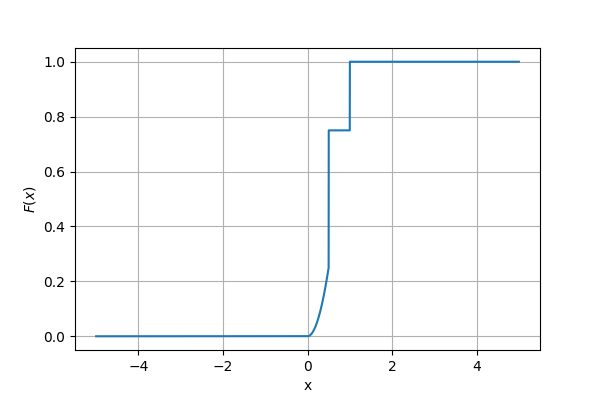
\includegraphics[width=\columnwidth]{solutions/ma/2016/30/figs/Assignment4_CDF.png}
\caption{The CDF of X}
\label{cdf}
\end{figure}



\item Let X and Y be continuous random variables with the joint probability density function 
\begin{align}
f\brak{x,y}= 
\begin{cases}
ae^{-2y} & 0<x<y<\infty \\
0 & \text{otherwise}.
\end{cases}   
\end{align}
Then $E\brak{X|Y=2}$ is \dots
\solution
Given X and Y are two continuous random variables with joint probability density function,
\begin{align}
f\brak{x,y}= 
\begin{cases}
ae^{-2y} & 0<x<y<\infty \\
0 & \text{otherwise}.
\end{cases}   
\end{align}
% \begin{figure}[!hbt]
%     \centering
%     \includegraphics[width=\columnwidth]{Figure_0.png}
%     \caption{Graph of x=y}
%     \label{Figure_1}
% \end{figure}
We know that,\\
$0<x<y<\infty  \implies x<y<\infty \text{ for } 0<x<\infty.$\\ 
Then,
\begin{align}
    f_X\brak{x} &= \int f_{XY}\brak{x,y}dy\\
    &= \int_{x}^{\infty} ae^{-2y}dy\\
    &= \left[ \frac{ae^{-2y}}{(-2)} \right]_{x}^{\infty}\\
    &= \frac{-a}{2}\left[ e^{-2y}\right]_{x}^{\infty}\\
    &= \frac{-a}{2}[0-e^{-2x}]\\
\implies f_X\brak{x} &=
    \begin{cases}
    \frac{a}{2}e^{-2x} & 0 < x < \infty\\
    0 & \text{otherwise}.
    \end{cases}
\end{align}
Similarly,\\
$ 0<x<y<\infty \implies 0<x<y \text{ for } 0<y<\infty$ \\
Then,
\begin{align}
    f_y\brak{y} &= \int f_{XY}\brak{x,y}dx\\
    &= \int_{0}^{y} ae^{-2y}dx\\
    &= ae^{-2y}[x]_{0}^{y}\\
    &= aye^{-2y}\\
\implies f_Y\brak{y} &=
    \begin{cases}
    aye^{-2y} & 0 < y < \infty\\
    0 & \text{otherwise}.
    \end{cases}
\end{align}
%\begin{figure}[ht]
%    \centering
%    \includegraphics[width=\columnwidth]{Figure_1.png}
%    \caption{Graph of x+y=1}
%    \label{Figure_1}
%\end{figure}
Therefore ,
\begin{align}
    f_{X|Y}\brak{x|y} &= \frac{f_{XY}\brak{x,y}}{f_Y\brak{y}}\\
    & = \frac{ae^{-2y}}{aye^{-2y}}\\
    & = \frac{1}{y}\\
\implies f_{X|Y}\brak{x|y} &=
    \begin{cases}
    \frac{1}{y} & \text{if } 0<x<y<\infty\\
    0 & \text{otherwise}
    \end{cases}
\end{align}
Then, 
\begin{align}
   E\brak{X|Y=y} & =
   \int_{-\infty}^{\infty} (x)f_{X|Y}\brak{x|y}dx\\
    & = \int_{0}^{y}(x)\brak{\frac{1}{y}}dx\\
    & = \frac{1}{y} \int_{0}^{y}(x)dx \\
    & = \frac{1}{y} \left[ \frac{x^2}{2}\right]_{0}^{y}\\
    & = \frac{1}{y}\brak{\frac{y^2}{2}}\\
    & = \frac{y}{2}\\
\implies E\brak{X|Y=y} &= \frac{y}{2}\\
\therefore E\brak{X|Y=2} &= 1
\end{align}
%
\item A continuous random variable X has the probability density function
\begin{align*}
    f(x) &= \begin{cases} 
      \frac{3}{5}e^{-\frac{3}{5}x} & x > 0 \\
      0 & x\leq 0\\
   \end{cases} 
\end{align*} 
The probability density function of $Y=3X+2$  is
\begin{enumerate}
    \item \begin{align*}
         f(y) &= \begin{cases} 
      \frac{1}{5}e^{-\frac{1}{5} (y-2)} & y > 2 \\
      0 & y \leq 2\\
   \end{cases} 
    \end{align*}
\item \begin{align*}
    f(y) &= \begin{cases} 
      \frac{2}{5}e^{-\frac{2}{5} (y-2)} & y > 2 \\
      0 & y \leq 2\\
   \end{cases} 
\end{align*} 
\item  \begin{align*}
    f(y) &= \begin{cases} 
      \frac{3}{5}e^{-\frac{3}{5} (y-2)} & y > 2 \\
      0 & y \leq 2\\
   \end{cases} 
\end{align*} 
\item \begin{align*}
    f(y) &= \begin{cases} 
      \frac{4}{5}e^{-\frac{4}{5} (y-2)} & y > 2 \\
      0 & y \leq 2\\
   \end{cases} 
\end{align*} 
\end{enumerate}
%
\solution
Given $Y=3X+2$ \\
    CDF of $Y$, 
    \begin{align*}
        F_y(Y) &= \Pr(Y\leq y) \\
        &= \Pr\left(X \leq \frac{y-2}{3} \right) \\
        &= F_x\left(\frac{y-2}{3}\right) \\
    \end{align*}
    Thus, pdf of $Y$ ,\begin{align*}
        f_Y(y) &= \frac{1}{3}f_X\left(\frac{y-2}{3}\right)\\
        &= \frac{1}{3} \times \begin{cases} \frac{3}{5}e^{-\frac{3}{5}\left(\frac{y-2}{3}\right)}  & y>2 \\
        0 & y \leq 2 \\\end{cases}\\
        &= \begin{cases} 
      \frac{1}{5}e^{-\frac{1}{5} (y-2)} & y > 2 \\
      0 & y \leq 2\\
   \end{cases} 
    \end{align*}
Hence, correct option is 1. 
%
\item    Let the probability density function of a random variable X be
   $$
   f(x)=
   \begin{cases}
   x~~~~~~~~~~~~~~~0\leqslant x < \dfrac{1}{2}\\
   c(2x-1)^2~~~~~\dfrac{1}{2}\leqslant x <1\\
   0 ~~~~~~~~~~~~~~~\text{Otherwise}
   \end{cases}
   $$
   Then value of c is equal to ...
   \\
\solution
We know that,
\begin{align}
\int_{-\infty}^{\infty}{f_x(x)}\,dx &= 1\\
    \int_{-\infty}^{0}{f_x(x)}\,dx +\int_{0}^{\frac{1}{2}}{f_x(x)}\,dx&\nonumber\\ +\int_{\frac{1}{2}}^{1}{f_x(x)}\,dx +\int_{1}^{\infty}{f_x(x)}\,dx&=1\\
    \int_{0}^{\frac{1}{2}}x\,dx+\int_{\frac{1}{2}}^{1}c(2x-1)^2\,dx&=1\\
    \sbrak{\dfrac{x^2}{2}}_0^\frac{1}{2}+c \sbrak{\dfrac{(2x-1)^3}{6}}_\frac{1}{2}^1&=1\\
    \dfrac{1}{8}+\dfrac{c}{6}&=1\\
    c&=\dfrac{21}{4}
\end{align}
\hspace{2cm}$\therefore$ Required value of $c=\dfrac{21}{4}$

\begin{figure}[h]
   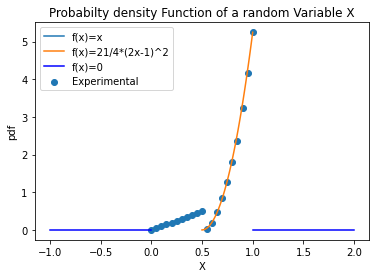
\includegraphics[width=\linewidth]{solutions/ma/2016/10/figures/plot.png}
    \caption{Experimental and Theoritical pdf of X}
    \label{fig:my_label}
\end{figure}




%
\item Let $A_{1},A_{2},.....A_{n}$ be n independent events in which the Probability of occurence of the event $A_{i}$ is given by P($A_{i}$) = 1 - $\frac{1}{\alpha^i}$, $\alpha >1$, i = 1,2,3,....n.Then the probability that atleast one of the events occurs is
\begin{enumerate}
    \item  1 - $\frac{1}{\alpha^\frac{n(n+1)}{2}}$ \hspace{0.95cm}
    \item  $\frac{1}{\alpha^\frac{n(n+1)}{2}}$\hspace{1.5cm}
    \\ \\
    \item  $\frac{1}{\alpha^n}$ \hspace{2.15cm}
    \item 1 - $\frac{1}{\alpha^n}$\hspace{0.95cm}
  \end{enumerate}
  %
  \solution
  Let $A_{1} + A_{2} + A_{3} .... + A_{n}$ = S, \\
$\pr{S}$ = Probability of atleast one event occuring
De morgan's law states that $(A + B)^\prime = A^\prime B^\prime$  
\begin{align}
    \label{1.1}
   \implies \pr{S} = 1 - \pr{S^\prime} \\ 
   %\label{1.2}
   1 - \pr{S^\prime}= 1 - \pr{A_{1}^\prime A_{2}^\prime A_{3}^\prime
   ....A_{n}^\prime}
   \label{ma2005:1}
\end{align}
$\forall$ i $\in$ {1,2,....n} \\
Since, $A_{i}$ are independent.\\
$\therefore$ Complements of $A_{i}$ are also independent.\\
$\implies$ 
\begin{equation}
%\label{2.1}
\pr{A_{1}^\prime A_{2}^\prime A_{3}^\prime
   ....A_{n}^\prime}=\prod_{i=1}^{n}\pr{A_{i}^\prime}
   \label{ma2005:2}
\end{equation}
\begin{equation}
%    \label{2.2}
\pr{A_{i}} = 1 - \frac{1}{\alpha^i} \implies \pr{A_{i}^\prime} = \frac{1}{\alpha^i} \label{ma2005:5}
\end{equation}
substituting \eqref{ma2005:5} in \eqref{ma2005:2},
\begin{equation}
    \label{2.3}
  \pr{A_{1}^\prime A_{2}^\prime A_{3}^\prime ....A_{n}^\prime} =  \prod_{i=1}^{n}\frac{1}{\alpha^i} \\
\end{equation}
\begin{equation}
\label{2.4}
   \prod_{i=1}^{n}\frac{1}{\alpha^i}=\frac{1}{\alpha^{\sum_{i}^{n}i}}= \frac{1}{\alpha^\frac{n(n+1)}{2}} 
\end{equation}
\begin{equation}
%\label{2.5}
    \therefore \pr{A_{1}^\prime A_{2}^\prime A_{3}^\prime ....A_{n}^\prime} = \pr{S^\prime} = \frac{1}{\alpha^\frac{n(n+1)}{2}} \label{ma2005:3}
\end{equation}
from equations \eqref{ma2005:1} and \eqref{ma2005:3} 
\begin{equation}
\label{2.6}
\implies \pr{S} = 1 - \pr{S^\prime} = 1 - \frac{1}{\alpha^\frac{n(n+1)}{2}}
\end{equation}
$\therefore$ The correct option is \textbf{(a)}
  %
  \item Let the random variable X have the distribution function 
$F(x)= \begin{cases}
       0  & if \:x<0\\
       \frac{x}{2} & if\: 0 \le x <1\\
       \frac{3}{5} & if \:1 \le x <2\\
       \frac{1}{2} +\frac{x}{8} & if\: 2\le x <3\\
       1  & if\: x\ge 3
    \end{cases}$\\
Then $\pr{2\le x <4}$ is equal to 
%
\\
  \solution
  
Given,
\begin{align}
F(x)= \begin{cases} 
       0  & if \:x<0\\
       \frac{x}{2} & if\: 0 \le x <1\\
       \frac{3}{5} & if \:1 \le x <2\\
       \frac{1}{2} +\frac{x}{8} & if\: 2\le x <3\\
       1  & if\: x\ge 3
    \end{cases} \label{a}
\end{align}
We need to find $\pr{2\le x <4}$,which is also can be written as
\begin{align}
\pr{2\le x <4} &= \pr{x<4} - \pr{ x <2}\\
              &= F(X=4^{-}) - F(X=2^{-})\label{b}
 \end{align} 
 Using \eqref{a} in \eqref{b},
 \begin{align}
 \pr{2\le x <4} &= 1 - \frac{3}{5}\\
                &= \frac{2}{5}\\
                &= 0.4 
\end{align} 


\begin{figure}[ht]
    \centering
    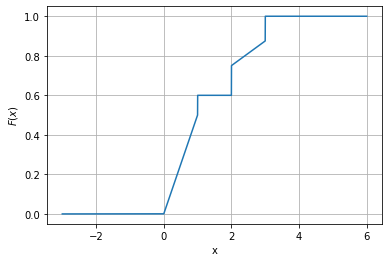
\includegraphics[width=\columnwidth]{solutions/ma/2015/9/Fig_assign_5.png}
    \caption{cdf of random variable X}
\end{figure}

\item Let Z be the vertical coordinate, between -1 and 1, of a point chosen uniformly at random on the
\begin{math}
\text{surface of a unit sphere in }R^3.\text{ Then,} \pr{\frac{-1}{2} \leq Z \leq \frac{1}{2}}
\end{math}
is
\\
  \solution
  The equation of the sphere can be written as :
\begin{math}
x^2 + y^2 + z^2 = 1.
\end{math}
Now,
\begin{align}
\pr{\frac{-1}{2} \leq z \leq 0}&=\pr{0 \leq z^2 \leq \frac{1}{4}}
\\\pr{0 \leq z \leq \frac{1}{2}}&=\pr{0 \leq z^2 \leq \frac{1}{4}}
\\\therefore \pr{\frac{-1}{2} \leq z \leq \frac{1}{2}}&=2 \times \pr{0 \leq z^2 \leq \frac{1}{4}}
\end{align}
\begin{align}
\pr{0 \leq z^2 \leq \frac{1}{4}}&=\pr{\frac{3}{4} \leq x^2+y^2 \leq 1}
\\\text{Taking, } x^2+y^2&=r^2.
\end{align}
\begin{align}
     \pr{\frac{3}{4} \leq r^2 \leq 1} &= \frac{1}{4}
\end{align}
     \brak{ \text{Since, }r^2 \text{ is uniform between 0 and 1} }
\begin{align}
     \therefore \pr{\frac{-1}{2} \leq Z \leq \frac{1}{2}} &= 2 \times \frac{1}{4} = \frac{1}{2}
\end{align}
%
\item Let $X_1$ and $X_2$ be independent geometric random variables with the same probability
mass function given by $\pr{X = k} = p(1-p)^{k-1}$
, $k = 1, 2, \ldots$ Then the value of
$\pr{X_1 = 2 | X_1 + X_2 = 4}$ correct up to three decimal places is
\\
  \solution
  Let 
\begin{align}
\label{eq:dice_pmf_xi}
p_{X_i}(k)=\pr{X_i=k}=
\begin{cases}
p(1-p)^{k-1} & n=1,2,...
\\
0 & otherwise
\end{cases}
\end{align}
where i=1,2
\begin{align}
\pr{A|B}=\frac{\pr{AB}}{\pr{B}}
\end{align}
\begin{align}
(X_1 = 2) \cap (X_1 + X_2 = 4)=\brak{X_1=2,X_2=2}
\end{align}
Thus,
\begin{align}
  \pr{X_1 = 2 | X_1 + X_2 = 4}&=\frac{\pr{X_1=2,X_2=2}}{\pr{X_1+X_2=4}}
 \end{align}
 Since the two events are independent,
\begin{align}\label{result}
  \pr{X_1 = 2 | X_1 + X_2 = 4}=\frac{\pr{X_1=2}\pr{X_2=2}}{\pr{X_1+X_2=4}}
 \end{align}
Let
\begin{align}\label{eq:dice_xdef}
X=X_1+X_2
\end{align}
From \eqref{eq:dice_xdef},
\begin{align}
p_X(n) &= \pr{X_1 + X_2 = n} = \pr{X_1  = n -X_2}
\\
&= \sum_{k}^{}\pr{X_1  = n -k | X_2 = k}p_{X_2}(k)
\label{eq:dice_x_sum}
\end{align}
after unconditioning.  $\because X_1$ and $X_2$ are independent,
\begin{multline}
\pr{X_1  = n -k | X_2 = k} 
\\
= \pr{X_1  = n -k}
= p_{X_1}(n-k)
\label{eq:dice_x1_indep}
\end{multline}
From \eqref{eq:dice_x_sum} and \eqref{eq:dice_x1_indep},
\begin{align}
p_X(n) = \sum_{k}^{}p_{X_1}(n-k)p_{X_2}(k) = p_{X_1}(n)*p_{X_2}(n)
\label{eq:dice_x_conv}
\end{align}
where $*$ denotes the convolution operation. 
%\cite{proakis_dsp}.  
Substituting from \eqref{eq:dice_pmf_xi}
in \eqref{eq:dice_x_conv},
\begin{align}
p_X(n)& = \sum_{k=1}^{n-1}p_{X_1}(n-k)p_{X_2}(k)\\
& = \sum_{k=1}^{n-1} (1-p)^{k-1} p \cdot (1-p)^{n-k-1} p \\ & = (1-p)^{n-2} p^2 \sum_{k=1}^{n-1} 1 \\& = (n-1) (1-p)^{n-2}p^2\label{ref}\end{align}
From \eqref{ref} and \eqref{eq:dice_pmf_xi} we have
\begin{align}
&\pr{X_1=2}=\pr{X_2=2}=p(1-p)\\
&\pr{X_1+X_2=4}=3(1-p)^2p^2
\end{align}
Substituting in \eqref{result}
\begin{align}
 \pr{X_1 = 2 | X_1 + X_2 = 4}
 &=\frac{(1-p)^2p^2}{3(1-p)^2p^2}\\
 &=\frac{1}{3}
\end{align}
%
\item     Let X and Y have joint probability function given by\\
    $$f_{X,Y}(x,y)=\left\{
    \begin{array}{ll}
      2 & 0\leq x\leq 1-y,0\leq y\leq 1 \\
      0 & otherwise \\
    \end{array} 
    \right. $$
    If $f_{Y}$ denotes the marginal probability density function of Y, then $f_{Y}(1/2)=?$
\\
\solution

\begin{align}
    \tag{23.1}
    f_{Y}(y) = \int_{-\infty}^{\infty}f_{X,Y}(x,y).dx
\end{align}
\begin{align}
    \tag{23.2}
    \implies f_{Y}(y) = \left\{
    \begin{array}{ll}
      0+\int_{0}^{1-y}2.dx & 0\leq y\leq 1 \\
      0 & otherwise \\
    \end{array} 
    \right.
\end{align}
\begin{align}
    \tag{23.3}
    \implies f_{Y}(y) = \left\{
    \begin{array}{ll}
      2(1-y) & 0\leq y\leq 1 \\
      0 & otherwise \\
    \end{array} 
    \right.
\end{align}
\begin{align}
    \tag{23.4}
    \therefore f_{Y}(1/2) = 1
\end{align}
\begin{figure}
\centering
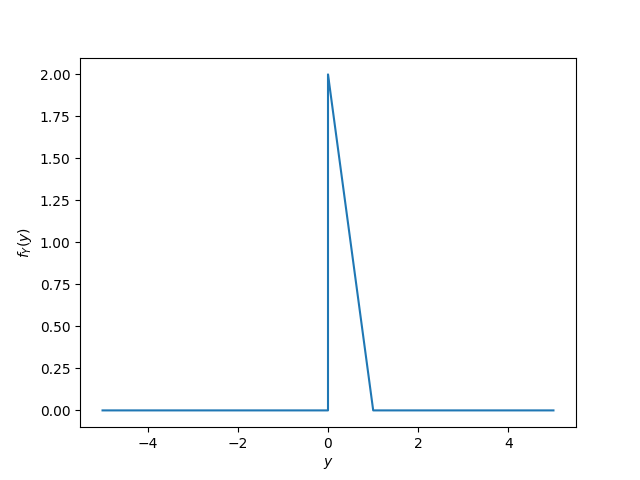
\includegraphics[width=\columnwidth]{solutions/ma/2018/23/Figure/Plot.png}
\caption{Marginal PDF}
\label{fig:ma2018-23:marginal}
\end{figure}



%
\item Let X be a standard normal random variable. Then $\pr{X < 0 |\;\abs{\lfloor X\rfloor} = 1}$ is equal to
\begin{enumerate}[label = \alph*)]
    \item $\cfrac{\Phi(1) - \frac{1}{2}}{\Phi(2) - \frac{1}{2}}$
    \item $\cfrac{\Phi(1) + \frac{1}{2}}{\Phi(2) + \frac{1}{2}}$
    \item $\cfrac{\Phi(1) - \frac{1}{2}}{\Phi(2) + \frac{1}{2}}$
    \item $\cfrac{\Phi(1) + 1}{\Phi(2) + 1}$
\end{enumerate}
%
\solution

\begin{align}
    &\abs{\lfloor X\rfloor} = 1\\
    \implies &\lfloor X\rfloor = 1\; or\; -1\\
    \implies &X \in [1, 2) \cup [-1, 0)
\end{align}
Here 
\begin{align*}
    \lfloor X\rfloor = greatest\; integer\; less\; than\; or\; equal\; to\; X
\end{align*}
Thus required probability
\begin{align}
    &= \frac{\pr{X\in [-1,0)}}{\pr{X \in [1, 2) \cup [-1, 0)}}
\end{align} 
Using symmetry of standard normal random variable about y = 0, we have required probability 
\begin{align}
    &= \cfrac{\pr{X\in (0,1]}}{\pr{X \in [1, 2) \cup (0, 1])}}\\
    &= \cfrac{\pr{X \in (0, 1]}}{\pr{X \in (0, 2)}}\\
    &= \cfrac{\pr{X < 1} - \pr{X < 0}}{\pr{X < 2} - \pr{X < 0}}\\
    &= \cfrac{\Phi(1) - \Phi(0)}{\Phi(2) - \Phi(0)}\\
    &= \cfrac{\Phi(1) - \frac{1}{2}}{\Phi(2) - \frac{1}{2}}\label{bato}\\
    &= \cfrac{0.841 - 0.5}{0.977 - 0.5}\label{gato}\\
    &= 0.715
\end{align}
Here $\Phi(x)$ represents the standard normal cumulative density function. Thus 
\begin{align}
    X \sim \mathcal{0}{1}
\end{align}
and 
\begin{align}
    \Phi(x) = \int_{-\infty}^x f_X(x)dx
\end{align}
It can easily be seen that $\Phi(0) = \frac{1}{2}$, which has been used to obtain \eqref{bato}.
\eqref{gato} was obtained by consulting tables for $\Phi(x)$
%
\item Let $X$ be a random variable with probability mass function 
$p(n) = \brak{\frac{1}{4}}\brak{\frac{3}{4}}^{n-1}  n=1,2 \ldots $ \\
Then $E[X-3|X>3]$ is \dots
\\
\solution

Given\begin{align}\label{ma2017-46:5}
\pr{X=n} = \begin{cases}
    \brak{\frac{1}{4}}\brak{\frac{3}{4}}^{n-1} & n=1,2 \ldots \\
    0 & otherwise
\end{cases}
\end{align}
Using the linearity of the expectation operator:
\begin{align}\label{ma2017-46:eq-1}
 E[X - 3 \mid X > 3] = E[X \mid X > 3] - 3
\end{align}
Now ,
\begin{align}
E[X \mid X > 3] &= \sum_{x=1}^{\infty} x  \pr{X=x \mid X > 3}\\
& = \sum_{x=1}^{\infty} x \frac{\pr{X=x, X > 3}}{\pr{X > 3}}\label{ma2017-46:eq1}
\end{align}
Calculating $\pr{X>3}$
\begin{align}
\pr{X > 3} =& 1 - \pr{X \leq 3}   \\
=& 1 - \sum_{x'=1}^3 \pr{X=x'} \\
=& 1 - \sum_{x'=1}^3 \brak{\frac{3}{4}}^{x'-1}\brak{\frac{1}{4}}\\
=& \frac{27}{64} \label{ma2017-46:eq2}
\end{align}
%Computing $P(X=x, X > 3)$
Also,\begin{align}\label{ma2017-46:eq3}
\pr{X=x, X > 3} = \begin{cases}
    \pr{X=x} & x > 3 \\
    0 & x \leq 3
\end{cases}
\end{align}
 %Combining the numerator and denominator
Substituting \eqref{ma2017-46:eq2} and \eqref{ma2017-46:eq3} in  \eqref{ma2017-46:eq1} we get
\begin{align}
E[X \mid X > 3] 
&= \sum_{x=1}^{3} 0 + \sum_{x=4}^{\infty} \sbrak{ x   \frac{\pr{X=x}}{\frac{27}{64}} } \\
&=\frac{64}{27} \sum_{x=4}^{\infty} \sbrak{  
x\brak{\frac{1}{4}}\brak{\frac{3}{4}}^{x-1}}\\
&=\frac{16}{27}\sum_{x=4}^{\infty} \sbrak{ x \brak{\frac{3}{4}}^{x-1}}\label{ma2017-46:sub}
\end{align}

Let
\begin{align}\label{ma2017-46:S}
S&=\sum_{x=4}^{\infty} \sbrak{ x \brak{\frac{3}{4}}^{x-1}}\
\end{align}
Multiplying (\eqref{ma2017-46:S}) with  $\frac{3}{4}$ on both sides gives
\begin{align}\label{ma2017-46:3/4S}
\frac{3}{4}S&=\sum_{x=4}^{\infty} x\frac{1}{4}\left(\frac{3}{4}\right)^{x} 
\end{align}
From \eqref{ma2017-46:3/4S} and\eqref{ma2017-46:S} 
\begin{align}
S&= 4 \brak{\frac{3}{4}}^{3}+5 \brak{\frac{3}{4}}^{4}+6 \brak{\frac{3}{4}}^{5}\ldots\\
\frac{3}{4}S&= 0\brak{\frac{3}{4}}^{3}+ 4 \brak{\frac{3}{4}}^{4}+5 \brak{\frac{3}{4}}^{5}+\ldots
\end{align}
subtracting \eqref{ma2017-46:3/4S} from \eqref{ma2017-46:S} we get
\begin{align}
\frac{S}{4}&= 4 \brak{\frac{3}{4}}^{3}+ \brak{\frac{3}{4}}^{4}+\brak{\frac{3}{4}}^{5}+\brak{\frac{3}{4}}^{6}+\ldots\\
&=4 \brak{\frac{3}{4}}^{3}+\sum_{x=4}^{\infty}   \brak{\frac{3}{4}}^{x}\\
&=\frac{189}{64}
\end{align}
Substituting vale of S in \eqref{ma2017-46:sub} we get
\begin{align}
    E[X|X>3]=7
\end{align}
Thus putting this in \eqref{ma2017-46:eq-1}
\begin{align}
    E[X-3|X>3]=4
\end{align}
\begin{figure}[h]
    \centering
    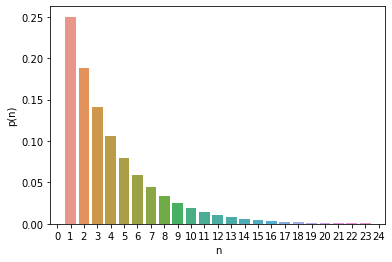
\includegraphics[width=\columnwidth]{solutions/ma/2017/46/figures/plot.png}
    \caption{PMF of $X$  }
    \label{ma2017-46:beta}
\end{figure}



%
\item Let (X,Y) be a random vector such that, for any $y>0$, the conditional probability density function of X given $Y=y$ is $$f_{X|Y=y}(x)=ye^{-yx} \:,x>0. $$ If the marginal probability density function of Y is $$g(y)=ye^{-y}\:,y>0$$ then $E(Y|x=1)=$
\\
\solution
Given,
the conditional probability density function of X given $Y=y$,
\begin{align}
f_{X|Y=y}(x)=ye^{-yx} \:,x>0 \label{st2020-43:a}
\end{align}
and, the marginal probability density function of Y,
\begin{align}
g(y)=ye^{-y}\:,y>0 \label{st2020-43:b}
\end{align}
let the joint probability density function of (X,Y) be $f_{X,Y}(x,y)$.
We know that,
\begin{align}
f_{X|Y=y}(x)=\frac{f_{X,Y}(x,y)}{g(y)}  \label{st2020-43:c}
\end{align}
using \eqref{st2020-43:a} and \eqref{st2020-43:b} in \eqref{st2020-43:c},
\begin{align}
f_{X,Y}(x,y) =y^{2}e^{-y(x+1)} \:,x,y>0 \label{st2020-43:d}
\end{align}
let the marginal probability density function of X be $f_{X}(x)$,
as we know ,
\begin{align}
f_{X}(x)= \int_{0}^{\infty}{f_{X,Y}(x,y)}\,dy \label{st2020-43:e}
\end{align}
using \eqref{st2020-43:d} in \eqref{st2020-43:e},
\begin{align}
f_{X}(x) &=\int_{0}^{\infty}{y^{2}e^{-y(x+1)}}\,dy\\
&=\frac{2}{(x+1)^{3}} \:,x>0\label{st2020-43:f}
\end{align}
The conditional probability density function of Y given $X=x$ is given by,
\begin{align}
f_{Y|X=x}(y) =\frac{f_{X,Y}(x,y)}{f_{X}(x)} \label{st2020-43:g}
\end{align}
using \eqref{st2020-43:d} and \eqref{st2020-43:f} in \eqref{st2020-43:g},
\begin{align}
 f_{Y|X=x}(y) =\frac{y^{2}e^{-y(x+1)}(x+1)^{3}}{2} \:,x,y>0
\end{align}
The conditional probability density function of Y given $X=1$ is given by,
\begin{align}
 f_{Y|X=1}(y) =4y^{2}e^{-2y}  \:,y>0 \label{st2020-43:h}
\end{align}
We need to find $E(Y|X=1)$ which is given by,
\begin{align}
 E(Y|X=1) &= \int_{0}^{\infty}{yf_{Y|X=1}(y)}\,dy \label{st2020-43:i}
\end{align}
using \eqref{st2020-43:h} in \eqref{st2020-43:i},
\begin{align}
E(Y|X=1) &= \int_{0}^{\infty}{4y^{3}e^{-2y}}\,dy\\
  &= \left[\frac{-e^{-2y}(8y^{3} + 12y^{2} + 12y + 6)}{4}\right]_0^{\infty}\\
        &=\frac{3}{2}
\end{align}

%
\item Let $X$ and $Y$ be jointly distributed random
variables having the joint probability
density function
\[
f(x,y) = \begin{cases}
            \frac{1}{\pi}, &\text{if}\quad x^2 + y^2 \leq 1\\
             0, &\text{otherwise}\\
            \end{cases}
\]
Then $\pr{Y > \text{max}(X,-X)}$ is
\\
\solution 

The pdf of $X$ and $Y$ are:
\begin{align}
    f_X(x)&=\int_{-\infty}^{\infty}f(x,y)dy\\
    &=\int_{-\sqrt{1-x^2}}^{\sqrt{1-x^2}}\frac{1}{\pi}dy\\
    &=\frac{2\sqrt{1-x^2}}{\pi}
\end{align}
\begin{align}
    f_Y(y)&=\int_{-\infty}^{\infty}f(x,y)dx\\
    &=\int_{-\sqrt{1-y^2}}^{\sqrt{1-y^2}}\frac{1}{\pi}dx\\
    &=\frac{2\sqrt{1-y^2}}{\pi}
\end{align}
The cdf of $Y$ is:
\begin{align}
    F_Y(y)&=\int_{-\infty}^{y}f_Y(y)dy\\
    &=\int_{-1}^{y}\frac{2\sqrt{1-y^2}}{\pi}dy\\
    &=\frac{2}{\pi}\left(\dfrac{\sin^{-1}{y} + y\sqrt{1-y^2}}{2} + \frac{\pi}{4}\right)
\end{align}
The value of $\pr{-X<Y<X}$ is:
\begin{align}
\pr{-X<Y<X} &=F_Y(X)-F_Y(-X)\\
 &=\frac{2}{\pi}\left(\sin^{-1}{X} + X\sqrt{1-X^2}\right)
\end{align}
Integrating our probability over all of $X$ we get the value of $ E[\pr{-x<Y<x}]$:
\begin{align}
&=\int_{-\infty}^{\infty}f_X(x)\pr{-x<Y<x}dx\\
    &=\left(\frac{2}{\pi}\right)^2\int_0^1\sqrt{1-x^2}\left(\sin^{-1}{x} + x\sqrt{1-x^2}\right)dx
\end{align}
Substituting
\begin{align} 
u &= \sin^{-1}{x} + x\sqrt{1-x^2}\\
\frac{du}{dx} &= 2\sqrt{1-x^2}\\
&=\left(\frac{2}{\pi}\right)^2\int_0^{\frac{\pi}{2}}\frac{u}{2}du\\
&=\left(\frac{2}{\pi}\right)^2\left(\frac{u^2}{4} \bigg |_0^{\frac{\pi}{2}}\right)\\
&=\left(\frac{2}{\pi}\right)^2\left(\frac{\pi^2}{16} - 0\right)\\
    &=\frac{4\cdot{\pi}^2}{{\pi}^2\cdot16}\\
    &=\frac{1}{4}
\end{align}
The probability for:
\begin{align}
    \pr{Y>\text{max}(X,-X)} = \frac{1}{4}
\end{align}
%
\item Let $X$ and $Y$ be two continuous random variables with the joint probability density function
\begin{align}
    f(x,y) =
    \begin{cases}
    2, & 0<x+y<1, x>0, y>0,\\
    0, & elsewhere.
    \end{cases}
\end{align}
$E\brak{X \bigm| Y=\frac{1}{2}}$ is
\begin{enumerate}
    \item $1/4$
    \item $1/2$
    \item $1$
    \item $2$
\end{enumerate}
\solution

The PDF of $X$ and $Y$ is,
\begin{align}
    f_X(x)=\int\limits_{-\infty}^\infty f(x,y)d y
\end{align}
\begin{align}
    f_X(x)=\int\limits_0^{1-x}2d y
\end{align}
\begin{align}
    f_X(x)=2-2x
\end{align}
\begin{align}
    f_Y(y)=\int\limits_{-\infty}^\infty f(x,y)d x
\end{align}
\begin{align}
    f_Y(y)=\int\limits_0^{1-y}2d x
\end{align}
\begin{align}
    f_Y(y)=2-2y
\end{align}
\begin{align}
    f_Y\brak{\frac{1}{2}}=1
\end{align}
by using Bayes theorem,
\begin{align}
    f_{X \mid Y}\brak{x \bigm| \frac{1}{2}}=\frac{f_{X,Y}\brak{x,\frac{1}{2}}}{f_Y\brak{\frac{1}{2}}}
\end{align}
\begin{align}
    f_{X\mid Y}\brak{x \bigm| \frac{1}{2}}=
    \begin{cases}
    2, & 0<x<\frac{1}{2},\\
    0, & elsewhere.
    \end{cases}
\end{align}
It is in the form of Bernoulli distribution, the expectation value is given by,
\begin{align}
    E\brak{X\bigm| Y=\frac{1}{2}}=\sum\limits_{-\infty}^{\infty}x f_{X\mid Y}\brak{x \bigm| \frac{1}{2}}
\end{align}
\begin{align}
    E\brak{X\bigm| Y=\frac{1}{2}}=\int\limits_{-\infty}^0x(0)d x + \int\limits_0^\frac{1}{2}x(2)d x + \int\limits^{-\infty}_0x(0)d x
\end{align}
\begin{align}
    E\brak{X\bigm| Y=\frac{1}{2}}=\int\limits_0^\frac{1}{2}2x d x
\end{align}
\begin{align}
    E\brak{X\bigm| Y=\frac{1}{2}}=\frac{1}{4}
\end{align}

%
\item An urn contains four balls, each ball having equal probability of being white or black. Three black balls are added to the urn. The probability that five balls in the urn are black is
\\
\solution

The total number of black balls are 5\\
Number of black balls initially present + number of black balls added =5\\
So, the number of black balls initially in the urn is 5-3=2\\
Let X be the random variable denoting the number of black balls in the urn. So, by binomial distribution, 
\begin{align}
    \pr{X=1}&=p\\
    \pr{X=k}&= {n\choose k} p^k (1-p)^{n-k}\\ \label{ma2018-11:eq}
    k&=0,1,2,...,n
\end{align}
For the given problem, $n=4$ and $p=0.5$, because there is equal probability for each ball of being white or black.
For having exactly 2 black balls, \\
From \eqref{ma2018-11:eq},
\begin{align}
    \pr{X=2}&= {4 \choose 2} \left(\frac{1}{2}\right)^2\left(\frac{1}{2}\right)^2\\
    &=\frac{6}{16}\\
    &=\frac{3}{8}
\end{align}
%
\item There are five bags each containing identical sets of ten distinct chocolates. One chocolate is picked from each bag.\\
The probability that at least two chocolates are identical is
%
\\
\solution

Let $X \in \{0,1,2,3,4,5\}$ represent the random variable, denoting the number of similar chocolates in the picked chocolates\\
Here, we can neglect X=1 because there can't be one similar object. \\
\begin{align}
    \pr{X\geq2}&+\pr{X=0}=1\\
    \pr{X=0}&=\frac{10.9.8.7.6}{10^5}\\
    \pr{X=0}&=0.3024\\
    \pr{X\geq 2}&=1-\pr{X=0}\\
    &=1-0.3024\\
    &=0.6976
\end{align}
%
Consider the trinomial distribution with the probability mass function 
\begin{multline}
    \nonumber \pr{X=x,Y=y}\\=\brak{\frac{7!}{x!y!(7-x-y)!}}(0.6)^x(0.2)^y(0.2)^{7-x-y}
\end{multline}
where $x\geq0 , y\geq0 \;and\; {x+y}\leq7$.
Then $E\brak{Y|X=3}$ is equal to
%
\\
\solution

Probability mass function of a trinomial  distribution is :
\begin{multline}
   \p{x}{y} \\=\brak{\frac{7!}{x!y!(7-x-y)!}}(0.6)^x(0.2)^y(0.2)^{7-x-y}\\
  \nonumber  =\brak{\frac{7!}{x!(7-x)!}\frac{(7-x)!}{y!(7-x-y)!}}(0.6)^x(0.2)^y(0.2)^{7-x-y}
\end{multline}
\begin{equation}
    \p{x}{y}=\comb{7}{x}\comb{7-x}{y}(0.6)^x(0.2)^y(0.2)^{7-x-y}\label{1}
\end{equation}
Using \eqref{1}, $\q{x}$ is 
\begin{align}
   \nonumber \q{x}&=\sum_{y=0}^{7-x} \p{x}{y}\\
  \nonumber &=\comb{7}{x}(0.6)^x\,\sum_{y=0}^{7-x}\, \comb{7-x}{y} (0.2)^y(0.2)^{7-x-y} \\
  \nonumber  &=\comb{7}{x}(0.6)^x\,{(0.4)^{7-x}}\\
    \q{x}&=\comb{7}{x}(0.6)^x\,{(0.4)^{7-x}}\label{2}
\end{align}
We have to find $\mean{Y|X=3}$ ,
\begin{align}
    \mean{Y|X=3}&=\sum_{y=0}^4 \: y P(Y=y|X=3)\\
    \mean{Y|X=3}&=\sum_{y=0}^4 y \brak{  \frac{ \p{3}{y}}{P(X=3)} }\label{3}
\end{align}
By taking X=3 in \eqref{1} and \eqref{2}  to use in \eqref{3},
\begin{align}
   \nonumber \mean{Y|X=3}&=\sum_{y=0}^4 y \brak{ \frac{ \p{3}{y}}{P(X=3)}}\\
  \nonumber  &=\sum_{y=0}^4 y   \brak{\frac{\comb{7}{3}\comb{4}{y}(0.6)^3(0.2)^y(0.2)^{4-y}}{\comb{7}{3}(0.6)^3\,{(0.4)^{4}}}}\\
 \nonumber &=\sum_{y=0}^4 y   \brak{\frac{\comb{4}{y}(0.2)^{4}}{{(0.4)^{4}}}}\\
 \mean{Y|X=3}&=\sum_{y=0}^4 {\frac{y(\comb{4}{y})}{{16}}}\label{4}
 \end{align}
 We know that,
 \begin{align}
     \comb{n}{r} = \frac{n}{r}\brak{\comb{n-1}{r-1}}\label{5}
 \end{align}
 Using \eqref{5} in \eqref{4},
 \begin{align}
  \mean{Y|X=3}&=\frac{1}{16}\sum_{y=0}^4\, {y(\comb{4}{y})}\\
  &=\frac{1}{16}\sum_{y=1}^{4} y\brak{\frac{4}{y}}(\comb{3}{y-1})\\
  &=\frac{1}{4}\sum_{k=0}^{3}(\comb{3}{k})\\
  &=\frac{1}{4}(1+1)^3=\frac{1}{4}(8)\\
  \mean{Y|X=3}&=2
\end{align}
Therefore the value of $\mean{Y|X=3}=2$.
\item Let E and F be any two events with $P(E \cup F) = 0.8$, $P(E) = 0.4$ and $P(E|F) = 0.3$ then P(F) is \newline
\begin{enumerate}
\item $\frac{3}{7}$ 
\item $\frac{4}{7}$ 
\item $\frac{3}{5}$ 
\item $\frac{2}{5}$ 
\end{enumerate}
%
\solution
%
Given,
\begin{align}
   \label{ma2010-1:(2.0.1)} \pr{E} &= 0.4 \\
   \label{ma2010-1:(2.0.2)} \pr{E+F} &= 0.8 \\
    \pr{E|F} &= 0.3
\end{align}
By definition,
\begin{align}
    \pr{E|F} &= \frac{\pr{EF}}{\pr{F}} \\
    \implies \pr{EF} &= \pr{E|F} \times \pr{F} \\
    \label{ma2010-1:(2.0.6)}\implies \pr{EF} &= 0.3 \times \pr{F}
\end{align}
Now using the identity,
\begin{align}
    \pr{E+F} &= \pr{E} + \pr{F} - \pr{EF}
\end{align}
From \eqref{ma2010-1:(2.0.1)},\eqref{ma2010-1:(2.0.2)} and \eqref{ma2010-1:(2.0.6)}
\begin{align}
    \implies 0.8 &= 0.4 + \pr{F} - \brak{0.3 \times \pr{F}} \\
    \implies 0.4 &= \brak{1-0.3} \times \pr{F} \\
    \implies \pr{F} &= \frac{0.4}{0.7}
\end{align}
\begin{equation}
    \boxed{\pr{F} = \frac{4}{7}}
\end{equation}
%
\item The number $N$ of persons getting injured in a bomb blast at a busy market place is a random variable having a Poisson Distribution with parameter $\lambda(\geq 1)$.
 A person injured in the explosion may either suffer a minor injury requiring first aid or suffer a major injury requiring hospitalisation. Let the number of persons with minor injury be $N_1$ and the conditional distribution of $N_1$ given N is
 \begin{align}
     \pr{N_1 = i \vert N} = \frac{1}{N}
     \label{condition}
 \end{align}
 Find the expected number of persons requiring hospitalisation.
 %
\solution
We know,
\begin{align}
    \pr{A|B} = \frac{\pr{A\cap B}}{\pr{B}}
\end{align}
Also, for a Poisson Distribution:
\begin{align}
    \pr{N = x} = \frac{e^{-\lambda}\lambda^x}{x!}
    \label{poisson}
\end{align}
where $\lambda$ is the parameter\\
Let $N_2$ be the number of persons hospitalised.\\
Let $N = a$, and $N_1 = i(i\leq a)$, then, $N_2 = a-i$\\
Then, from \eqref{condition} and \eqref{poisson}:
\begin{align}
    \pr{N_2 = a-i} =\pr{N_1 = i}\\
    =\pr{N_1 = i|N = a}\pr{N = a}\\
     = \frac{1}{a}\frac{e^{-\lambda}\lambda^a}{a!}
\end{align}
Thus,
\begin{align}
    E(N_2) = \sum_{a = 0}^{\infty} \sum_{i = 0 }^{a} (a-i) \times \frac{1}{a}\frac{e^{-\lambda}\lambda^a}{a!}\\
     = \sum_{a=0}^{\infty}\frac{e^{-\lambda}\lambda^a}{a!} \sum_{i = 0 }^{a} \frac{a-i}{a}\\
    = \sum_{a=0}^{\infty}\frac{e^{-\lambda}\lambda^a}{a!} \brak{a - \frac{(a+1)}{2}}\\
     = \sum_{a=0}^{\infty}\frac{e^{-\lambda}\lambda^a}{a!}\frac{a-1}{2}\\
      = \frac{e^{-\lambda}}{2}\sbrak{\sum_{a=0}^{\infty}\frac{a\lambda^a}{a!} - \sum_{a=0}^{\infty}\frac{\lambda^a}{a!}}\\
       = \frac{e^{-\lambda}}{2}\sbrak{\lambda\sum_{a=1}^{\infty} \frac{\lambda^{a-1}}{(a-1)!} - \sum_{a=0}^{\infty}\frac{\lambda^a}{a!}}\\
        = \frac{e^{-\lambda}}{2}\sbrak{\lambda e^\lambda - e^\lambda}\\
         = \frac{\lambda - 1}{2}
\end{align}
 %
 \item The time to failure, in months, of lights bulbs \\manufactured at two plants A and B
obey the exponential distributions with means 6 and 2 months respectively. Plant B produces
four times as many bulbs as plant A does. Bulbs from these two plants are indistinguishable.
They are mixed and sold together. Given that a bulb purchased at random is working after 12 months, What is the probability that it was manufactured in plant A?
\\
\solution

This problem involves Bayes theorem and \newline Exponential distribution
\bigskip
\begin{itemize}
    \item Probability that bulb is from Plant A =\newline $\pr{A}$ = \(\frac{1}{5}\)
    \item Probability that bulb is from Plant B =\newline$\pr{B}$ = \( \frac{4}{5} \)
\end{itemize}
\bigskip
One can use exponential distribution to find out the probability that the bulbs work after 12 months\\
Let X be a variable representing the lifetime of a bulb in months.\\
So X has a Cumulative distribution Function:
\begin{equation}
    F_X(x,\lambda) =
    \begin{cases}
        1 - {e}^{-\displaystyle\lambda x} & if \hspace{0.3cm}x \geq 0 \\
        0                                 & if \hspace{0.3cm}x < 0
    \end{cases}
\end{equation}
\begin{table}[!ht]
    \begin{center}
        \resizebox{\columnwidth}{!}
        {
            \begin{tabular}{|c|c|}
                \hline
                $\frac{1}{\displaystyle\lambda}$ &  Mean of distribution\\
                \hline
                x & Time to failure (in months)\\
                \hline
                $\lambda_A$ & $\frac{1}{6}$\\
                \hline
                $\lambda_B$ & $\frac{1}{2}$\\
                \hline
                $\pr{X\leq k}$ & $F_X(X,\lambda)$\\
                \hline
            \end{tabular}
        }
    \end{center}
\end{table}
Let us denote that the bulbs works after 12 months with the variable W.
\begin{align}
\text{$\pr{W \mid A}$} = & 1 -\notag \text{Pr(Fails within 12 months $\mid$ A)}\\
    = & 1 - F_X(12,\lambda_A)                       \\
    = & {e}^{\displaystyle - \lambda_A \times 12} 
\end{align}
\begin{align}
    \text{$\pr{W \mid B}$} = & 1 -\notag \text{Pr(Fails within 12 months $\mid$ B)}\\
        = & 1 - F_X(12,\lambda_B)                       \\
        = & {e}^{\displaystyle - \lambda_B \times 12} 
\end{align}
From Bayes theorem,\\
\begin{align}
    \pr{A \mid W} = & \displaystyle{\frac{Pr(A) \times Pr(W \mid A)}{Pr(A) \times Pr(W \mid A) + Pr(B) \times Pr(W \mid B)}}\\
    = & \displaystyle{\frac{Pr(A) \times {e}^{\displaystyle - \lambda_A \times 12}}{Pr(A) \times {e}^{\displaystyle - \lambda_A \times 12} + Pr(B) \times {e}^{\displaystyle - \lambda_B \times 12} }}
\end{align}
Substituting the known values, we get
\begin{align}
    \pr{A \mid W} = &\displaystyle{\frac{\displaystyle{\frac{1}{5}} \times {e}^{\displaystyle - 2}}{\displaystyle{\frac{1}{5}} \times {e}^{\displaystyle - 2} + \displaystyle{\frac{4}{5}} \times {e}^{\displaystyle - 6} }}\\[0.4cm]
    = & 0.93173845935
\end{align}
So the probability that the Bulb is manufactured in Plant A given that it works after a year is 0.93173845935.
 %
\item The lifetime of two brands of bulbs X and Y are exponentially distributed with the mean life of 100 hours. Bulb X is switched on 15 hours after bulb Y has been switched on. The probability that bulb X fails before bulb Y is 
\begin{enumerate}[label=(\Alph*)]
    \item $\frac{15}{100}$ \\
    \item $\frac{1}{2}$ \\
    \item $\frac{85}{100}$ \\
    \item 0 
  \end{enumerate}
  \solution
  Let X and Y be exponential random variables which represent the lifetime of bulbs X and Y respectively, both with mean = 100.\\
Using memorylessness property for exponential distribution, which states that :\\
\emph{An exponentially distributed random variable T obeys the relation}
\begin{align}
  \pr{T>t+s |T>s} = \pr{T>t}
\end{align} 
\emph{where $s,t\geq 0$}\\
Proof : Using Complementary cumulative distributive function, we get
\begin{align}
   \pr{T>t+s |T>s} =& \frac{\pr{T>t+s , T>s}}{\pr{T>s}} \\
   =& \frac{\pr{T>t+s}}{\pr{T>s}} \\
   =& \frac{e^{-\lambda(t+s)}}{e^{-\lambda s}}\\
   =&  e^{-\lambda t}\\
   =& \pr{T>t}
\end{align}
Probability that bulb X fails before bulb Y given that bulb Y was functioning when bulb X was switched on 
\begin{align}
  \pr{Y>X+15 | Y \geq 15}
  =& \pr{Y>X}
\end{align}
For both X and Y,
\begin{equation}
\lambda= \frac{1}{100} = 0.01
\end{equation}
\\
Probability distribution function of exponential random variables is given by : 
For x,y $\geq$ 0
\begin{align}
    \texorpdfstring{f\textsubscript{X}}{f X}(x) = \lambda e^{-\lambda x}\\
    \texorpdfstring{f\textsubscript{Y}}{f Y}(y) = \lambda e^{-\lambda y}
\end{align}
Cumulative distribution function of exponential random variables is given by : 
For x $\geq$ 0
\begin{align}
    \texorpdfstring{F\textsubscript{X}}{F X}(x) = 1- e^{-\lambda x}\\
    \texorpdfstring{F\textsubscript{Y}}{F Y}(x) = 1- e^{-\lambda x}
\end{align}
\begin{align}
    \pr{Y>X} =& \int_{-\infty}^{\infty}  \texorpdfstring{F\textsubscript{Y}}{F Y}(x) \texorpdfstring{f\textsubscript{X}}{f X}(x)  dx\\
    =& \int_{0}^{\infty} ( 1- e^{-\lambda x}) \lambda e^{-\lambda x}\\
    =&  \lambda \brak{\frac{1}{2\lambda} e^{-2\lambda x} - \frac{1}{\lambda} e^{-\lambda x}} \Bigg|_0^\infty\\
     =& \brak{\frac{1}{2} e^{-2\lambda x} - e^{-\lambda x}} \Bigg|_0^\infty\\
    =& \brak{\frac{1}{2} e^{-0.02x} - e^{-0.01x}} \Bigg|_0^\infty\\
    =& \frac{1}{2} = 0.5
\end{align}
 $\therefore$The answer is option (b) \large $\frac{1}{2}$.

  %
  \item Let $X_{1},X_{2},\dots$, be a sequence of independent and identically distributed random variables with $P(X_{1}=1)=\dfrac{1}{4}$ and $P(X_{1}=2)=\dfrac{3}{4}$. If $\bar X_{n}=\dfrac{1}{n}\displaystyle\sum_{i=1}^{n}X_{i}$,  for $n=1,2,\dots$, then $\displaystyle\lim_{n\to\infty}P(\bar X_{n} \leq 1.8)$ is equal to
  \\
  \solution
  
Given,
\begin{align}
\tag{32.1}
    Pr(X_{1}=1)=\dfrac{1}{4},Pr(X_{2}=2)=\dfrac{3}{4}
\end{align}
As $X_{1},X_{2},\dots$, are identically distributed random variables, $\forall i \in \{1,2,\dots,n\}$
\begin{align}
\tag{32.2}
    Pr(X_{i}=1)=\dfrac{1}{4},Pr(X_{i}=2)=\dfrac{3}{4}
\end{align}
Also,
\begin{align}
\tag{32.3}
    \because P(X_{i}&=1)+P(X_{i}=2)=1\\
\tag{32.4}
    &\therefore X_{i} \in \{1,2\}
\end{align}
Therefore, each $X_{i}$ is a bernoulli distribution with
\begin{align}
\tag{32.5}
    p=\dfrac{3}{4},q=\dfrac{1}{4}
\end{align}
Let
\begin{align}
\tag{32.6}
    X=\displaystyle\sum_{i=1}^{n}X_{i}
\end{align}
be a binomial distribution. Its CDF is
\begin{align}
\tag{32.7}
    Pr(X\leq n+r)=\displaystyle\sum_{k=0}^{r}{\comb{n}{k}}p^{k}q^{n-k}
\end{align}
To find : $\displaystyle\lim_{n\to\infty}Pr(\bar X_{n} \leq a)$
\begin{align}
\tag{32.8}
    \bar X_{n} \leq a \Rightarrow X \leq na
\end{align}
Substituting $a(=1.8),p,q$, we get
\begin{align}
\tag{32.9}
    \displaystyle\lim_{n\to\infty}Pr(\bar X_{n} \leq 1.8)&=\displaystyle\lim_{n\to\infty}P(X\leq 1.8n)\\
\tag{32.10} 
    &=\displaystyle\sum_{k=0}^{0.8n}\dfrac{{\comb{n}{k}}3^{k}}{4^{n}}
\label{eq:val}
\end{align}
On solving \eqref{eq:val}, we get
\begin{align}
\tag{32.11}
    \displaystyle\lim_{n\to\infty}P(\bar X_{n} \leq 1.8)=1
\end{align}

  %
  \item Let $X$ be the number of heads in 4 tosses of a fair coin by Person 1 and let $Y$ be the number of heads in 4 tosses of a fair coin by Person 2. Assume that all the tosses are independent. Then the value of $\Pr{(X=Y)}$ correct up to three decimal places is $\rule{1.6cm}{0.15mm}$ .
%
  \solution
  %
Let $X \in \{ 0, 1, 2, 3, 4\}$ be the random variable representing the number of heads obtained by Person 1 in 4 tosses. Similarly, Let $Y \in \{ 0, 1, 2, 3, 4\}$ be the random variable representing the number of heads obtained by Person 2 in 4 tosses. Then $X \text{ and } Y$ are binomial distributions with parameter:
\begin{align}
    p = \frac{1}{2}
\end{align}
Then,
\begin{align}
    \Pr(X=i) = 
	\begin{cases}
	\comb{4}{k}(p)^k(1-p)^{4-k} &  i \in \{0, 1, 2, 3, 4\}\\ 
	0 & \text{otherwise}
	\end{cases}
	\\\Pr(X=i) = 
	\begin{cases}
	\comb{4}{k}(\frac{1}{2})^k(1-\frac{1}{2})^{4-k}  &  i \in \{0, 1, 2, 3, 4\}\\ 
	0 & \text{otherwise}
	\end{cases}
	\\\Pr(X=i) = 
	\begin{cases}
	\comb{4}{k}\times(\frac{1}{2})^4  &  i \in \{0, 1, 2, 3, 4\}\\ 
	0 & \text{otherwise}
	\end{cases}
\end{align}
\begin{center}
\begin{table}[h]
    \centering
    \resizebox{\columnwidth}{!}{
\begin{tabular}{|c|c|c|}
\hline
Serial number & Case & Probability of the case \\
\hline
1 & $\Pr(X=0)$ & $\frac{\comb{4}{0}}{16} = \frac{1}{16}$ \\ 
\hline
2 & $\Pr(X=1)$ & $\frac{\comb{4}{1}}{16} = \frac{4}{16}$ \\ 
\hline
3 & $\Pr(X=2)$ & $\frac{\comb{4}{2}}{16} = \frac{6}{16}$ \\
\hline
4 & $\Pr(X=3)$ & $\frac{\comb{4}{3}}{16} = \frac{4}{16}$ \\
\hline
5 & $\Pr(X=4)$ & $\frac{\comb{4}{4}}{16} = \frac{1}{16}$ \\
\hline
\end{tabular}
}
    \caption{Probability distribution table of X}
    \label{table 1}
\end{table}
\end{center}
Similar is the distribution of $Y$. For finding $\Pr{(X=Y)}$, let $Y=y$,
\begin{align}
    \Pr{(X=Y)} = \frac{\comb{4}{y}}{16} \times \Pr{(Y=y)}
\end{align}
Generalizing this result,
\begin{align}
    \Pr{(X=Y)} &= \sum_{y=0}^4  \frac{\comb{4}{y}}{16}\times \Pr{(Y=y)}
    \\ &= \sum_{y=0}^4 \frac{\comb{4}{y}}{16} \times \frac{\comb{4}{y}}{16}
\end{align}
\begin{multline}
    \Pr{(X=Y)} = \brak{\frac{1}{16}\times\frac{1}{16}} + \brak{\frac{4}{16}\times\frac{4}{16}} +\brak{\frac{6}{16}\times\frac{6}{16}} \\+\brak{\frac{4}{16}\times\frac{4}{16}} +\brak{\frac{1}{16}\times\frac{1}{16}} 
\end{multline}
\begin{align}
    \Pr{(X=Y)} &= \frac{1}{256} + \frac{16}{256} +\frac{36}{256} +\frac{16}{256} +\frac{1}{256} 
    \\&= \frac{70}{256} 
    \\&= \frac{35}{128} 
    \\&= 0.2734375
\end{align}
\item The probability density function of a random variable X is
\begin{equation}
f(x)=
\begin{cases}
\frac{1}{\lambda}e^{\brak{-\frac{x}{\lambda}}}, & x>0\\
0, & x\leq 0
\end{cases}
\end{equation}
where $\lambda>0.$ For testing the hypothesis $H_{0}:\lambda=3$ against $H_{1}:\lambda=5$, a test is given as "Reject $H_0$ if $X\geq 4.5$".The probability of type 1 error and power of the test are respectively: 
\begin{enumerate}
\begin{multicols}{2}
\setlength\itemsep{1em}
\item 0.1353 and 0.4966\\
\item 0.1827 and 0.379\\
\item 0.2021 and 0.4493\\
\item 0.2231 and 0.4066
\end{multicols}
\end{enumerate}
%
  \solution
  %
\begin{definition}
\label{Type 1 error}A type 1 error occurs if the null hypothesis $H_{0}$ is rejected even if it is true.
\end{definition}
\begin{definition}
\label{Power of the test}The probability that the alternative hypothesis $H_{1}$ is true is defined to be Power of a given test. 
\end{definition}
Given,
\begin{equation}
f_{X}(x)=
\begin{cases}
\frac{1}{\lambda}e^{\brak{-\frac{x}{\lambda}}}, & x>0\\
0, & x\leq 0
\end{cases}
\end{equation}
Let cumulative distribution function be $F_{X}(x)$ for a given $\lambda$.
Hence,
\begin{equation}
    F_{X}(x)=\int_{-\infty}^{x}f_{X}(a) da
\end{equation}
From the probability density function,
\begin{align}
    \implies F_X(4.5)&=\int_{-\infty}^{x}f_{X}(a) da\\
    &=\int_{0}^{4.5}\frac{1}{\lambda}e^{\brak{-\frac{a}{\lambda}}}da\\
    &=1-e^{-\frac{4.5}{\lambda}}
\end{align}
We need the probability for $X\geq 4.5$,hence required probability is,
\begin{align}
1-F_{X}(4.5)=e^{-\frac{4.5}{\lambda}}\label{eq:2.0.6}
\end{align}
From \eqref{eq:2.0.6} we get probability that the given null hypothesis$(H_{0})$ is true is,
\begin{align}
e^{-\frac{4.5}{3}}=0.2231.
\end{align}
$\therefore$ The \textbf{probability of type 1 error is 0.2231}.
From \eqref{eq:2.0.6},we get the required probability that the given alternative hypothesis($H_{1}$) is true is,
\begin{align}
e^{-\frac{4.5}{5}}=0.4066
\end{align}
$\therefore$ The \textbf{power of the test is 0.4066}

  %
  \item  Let $E$ and $F$ be any two events with $\pr{E}=0.4, \pr{F}=0.3$
and $\pr{F|E}=3 \pr{F|E'}$. Then $\pr{E|F}$ equals ......
\\
  \solution
  Given
\begin{enumerate}
\item $\pr{E}=0.4$
\item $\pr{F}=0.3$
\item $\pr{F|E}=3 \pr{F|E'}$
\end{enumerate}
From given data
\begin{align}
\pr{F|E}=3 \pr{F|E'}\\
\frac{\pr{FE}}{\pr{E}}=3\times \frac{\pr{FE'}}{\pr{E'}}\\
\pr{EF}=2\times\pr{E'F}\label{eq:fac}
\end{align}
We know that
\begin{align}
\pr{F}=\pr{EF}+\pr{E'F} \label{eq:refer}
\end{align}
Using \eqref{eq:fac} and \eqref{eq:refer}, we get
\begin{align}
\pr{F}=\frac{3}{2}\times\pr{EF}\\
\frac{\pr{EF}}{\pr{F}}=\frac{2}{3}\\
\pr{E|F}=\frac{2}{3}\approx 0.66
\end{align}
%
\item Let a random variable $X$ follow the exponential distribution with mean 2. Define $Y$ such that:
\begin{align}
   Y =  \left[X-2\right|X>2]\nonumber
\end{align}
Then $E(Y)$ is equal to:\\
\\(A) $\frac{1}{4}$\\
\\(B) $\frac{1}{2}$\\
\\(C) 1\\
\\(D) 2\\
\item If A and B are two events and the probability $\Pr(B) \neq 1$,then\\
\begin{equation}
    \frac{\Pr(A)-\Pr(A \cap B)}{1-\Pr{(B)}}
\end{equation}
equals
\begin{enumerate}
\begin{multicols}{2}
\setlength\itemsep{1em}
\item $\Pr{(A|\bar{B})}$\\
\item $\Pr{(A|B)}$\\
\item $\Pr{(\bar{A}|B)}$\\
\item $\Pr{(\bar{A}|\bar{B})}$
\end{multicols}
\end{enumerate}
  \solution
  
Given A and B are two events,\\
We know that,
\begin{align}
    A&=A(B+\bar{B})\\
    &=AB+A\bar{B}
\end{align}
Since $AB$ and $A\bar{B}$ are disjoint events,
\begin{align}
    \Pr{(A)}=\Pr{(AB)}+\Pr{(A\bar{B})}
\end{align}
Hence,
\begin{equation}
    \Pr(A\bar{B})=\Pr{(A)}-\Pr{(AB)}\label{ma1997-18:eq:2.0.4}
\end{equation}
Since $B$ and $\bar{B}$ are disjoint events,
\begin{align}
    \Pr{(B)}+\Pr{(\bar{B})}=1\\
    \Pr{(\bar{B})}=1-\Pr{(B)}\label{ma1997-18:eq:2.0.6}
\end{align}
We know that,
\begin{equation}
\Pr{(A|\bar{B})}=\frac{\Pr{(A\bar{B})}}{\Pr{(\bar{B})}} \label{ma1997-18:eq:2.0.7}    
\end{equation}
From \eqref{ma1997-18:eq:2.0.6} and \eqref{ma1997-18:eq:2.0.4}
\begin{align}
    \frac{\Pr(A)-\Pr(AB)}{1-\Pr{(B)}}=\frac{\Pr{(A\bar{B})}}{\Pr{(\bar{B})}}
\end{align}
From \eqref{ma1997-18:eq:2.0.7}
\begin{equation}
    \frac{\Pr(A)-\Pr(AB)}{1-\Pr{(B)}}=\Pr{(A|\bar{B})}
\end{equation}
Hence \textbf{option A is correct}
%
\item If a random variable X assumes only positive integral values ,with the probability
\begin{equation}
 P(X=x)=\frac{2}{3}\brak{\frac{1}{3}}^{x-1},x=1,2,3,....,   
\end{equation}
then $E(X)$ is 
\begin{enumerate}
\begin{multicols}{2}
\item $ \frac{2}{9}$\\
\item $\frac{2}{3}$\\
\item $ 1$\\
\item $\frac{3}{2}$
\end{multicols}
\end{enumerate}
  \solution
  %
  Given that random variable X  assumes only positive integral values and its probability is:
  \begin{align}
      P(X=x)=\frac{2}{3}\brak{\frac{1}{3}}^{x-1}
  \end{align}
  The expectation value E(X) is given by 
  \begin{align}
      E(X)=\sum_{i=1}^{\infty} i \times P(X=i)
  \end{align}
  Let $E(X)=S$\\
  so,
  \begin{align}
      S&=\sum_{i=1}^{\infty} i \times P(X=i)\\
    \implies S&=\sum_{i=1}^{\infty} i \times
      \frac{2}{3}\brak{\frac{1}{3}}^{i-1}\label{ma2012-29:eq:0.0.5}\\
     \implies S&=\frac{2}{3}+\sum_{i=2}^{\infty} i \times
      \frac{2}{3}\brak{\frac{1}{3}}^{i-1}\label{ma2012-29:eq:0.0.6}
  \end{align}
  As
  \begin{align}
      \sum_{i=2}^{\infty} i \times
      \frac{2}{3}\brak{\frac{1}{3}}^{i-1}=\sum_{i=1}^{\infty} (i+1)\times
      \frac{2}{3}\brak{\frac{1}{3}}^{i}\label{ma2012-29:eq:0.0.7}
  \end{align}
  Now substituting  \eqref{ma2012-29:eq:0.0.7} in \eqref{ma2012-29:eq:0.0.6}
  \begin{align}
      \implies S&=\frac{2}{3}+\sum_{i=1}^{\infty} (i+1) \times
      \frac{2}{3}\brak{\frac{1}{3}}^{i}
  \end{align}
  \begin{align}
       \implies S&=\frac{2}{3}+\sum_{i=1}^{\infty} i \times
      \frac{2}{3}\brak{\frac{1}{3}}^{i}+\sum_{i=1}^{\infty} 
      \frac{2}{3}\brak{\frac{1}{3}}^{i}\label{ma2012-29:eq:0.0.9}
  \end{align}
   Dividing with 3 on both sides in \eqref{ma2012-29:eq:0.0.5} gives
   \begin{align}
      \frac{S}{3}=\sum_{i=1}^{\infty} i \times
      \frac{2}{3}\brak{\frac{1}{3}}^{i}\label{ma2012-29:eq:0.0.10}
  \end{align}
  Now substituting \eqref{ma2012-29:eq:0.0.10} in \eqref{ma2012-29:eq:0.0.9} gives
  \begin{align}
     \implies S&=\frac{2}{3}+\frac{S}{3}+\sum_{i=1}^{\infty}\frac{2}{3}\brak{\frac{1}{3}}^{i}
     \end{align}
     \begin{align}
     \implies \frac{2S}{3}&=\frac{2}{3}+\frac{2}{3}\sum_{i=1}^{\infty}\brak{\frac{1}{3}}^{i}
  \end{align}
  \begin{align}
     \implies \frac{2S}{3}&=\frac{2}{3}\brak{
     1+\sum_{i=1}^{\infty}\brak{\frac{1}{3}}^{i}}
  \end{align}
  \begin{align}
     \implies S=1+\sum_{i=1}^{\infty}\brak{\frac{1}{3}}^{i}
  \end{align}
  \begin{align}
     \implies S=1+\frac{\frac{1}{3}}{1-\frac{1}{3}}
  \end{align}
  \begin{align}
     \implies S=1+\frac{1}{2}=\frac{3}{2}
  \end{align}
  \begin{align}
     \implies E(X)=S=\frac{3}{2}
  \end{align}
  %
  \textbf{$\therefore$ Option D is correct}    
%
\item Let $X ,Y$ be continuous random variables with joint density function
\begin{align*}
    f_{X,Y}(x,y)=\begin{cases}
    e^{-y}(1-e^{-x}) \text{   if } 0< x<y<\infty\\
    e^{-x}(1-e^{-y}) \text{   if } 0< y\leq x<\infty
    \end{cases}
\end{align*}
Then The value of $E[X+Y]$ is 
%
\solution
  Let $g(X,Y)=X+Y$
We know that,
\begin{align*}
    &E[g(X,Y)]=\int_{-\infty}^{+\infty}\int_{-\infty}^{+\infty}g(x,y)f_{X,Y}(x,y)dxdy\\
\end{align*}
Then,
\begin{align*}
    &E[X+Y]=\int_{-\infty}^{+\infty}\int_{-\infty}^{+\infty}(x+y)f_{X,Y}(x,y)\,dxdy\\
    &=\int_{0}^{+\infty}\int_{0}^{+\infty}(x+y)f_{X,Y}(x,y)\,dxdy\\
    &=\int_{0}^{+\infty}\left(\int_{0}^{+\infty}xf_{X,Y}(x,y)\,dx+\int_{0}^{+\infty}yf_{X,Y}(x,y)\,dx\right)\,dy
\end{align*}
First we will calculate the $\int_{0}^{+\infty}yf_{X,Y}(x,y)\,dx$,  $\int_{0}^{+\infty}xf_{X,Y}(x,y)\,dx$ seperately.\\
consider,
\begin{align*}
    &\int_{0}^{+\infty}yf_{X,Y}(x,y)\,dx\\
    &=\int_{0}^{y}ye^{-y}(1-e^{-x})\,dx+\int_{y}^{+\infty}ye^{-x}(1-e^{-y})\,dx\\
    &=(ye^{-y})(y+e^{-y}-1)+y(1-e^{-y})e^{-y}\\
    &=y^2e^{-y}
\end{align*}
So,
\begin{align}
    \tag{37.1}
    \int_{0}^{+\infty}yf_{X,Y}(x,y)\,dx=y^2e^{-y}
\end{align}
Now consider,
\begin{align*}
  &\int_{0}^{+\infty}xf_{X,Y}(x,y)\,dx\\
  &=\int_{0}^{y}xe^{-y}(1-e^{-x})\,dx+\int_{y}^{+\infty}xe^{-x}(1-e^{-y})\\
  &=e^{-y}\left(\frac{y^2}{2}+e^{-y}(y+1)-1\right)+(1-e^{-y})(e^{-y}(y+1))\\
  &=\frac{y^2e^{-y}}{2}+ye^{-y}
\end{align*}
So,
\begin{align}
    \tag{37.2}
    \int_{0}^{+\infty}xf_{X,Y}(x,y)\,dx=\frac{y^2e^{-y}}{2}+ye^{-y}
\end{align}
From Eq 37.1 and 37.2
\begin{align*}
    &E[X+Y]=\int_{0}^{+\infty}\left(\frac{y^2e^{-y}}{2}+ye^{-y}+y^2e^{-y}\right)\,dy\\
    &=\int_{0}^{+\infty}\left(\frac{3}{2}y^2e^{-y}+ye^{-y}\right)\,dy\\
    &=\left(-\frac{3}{2}(y^2+2y+2)e^{-y}+(-e^{-y}(y+1))\right)\Biggr|_{0}^{+\infty}\\
    &=\frac{3}{2}\times2+1\\
    &=4
\end{align*}
So,
\begin{align*}
  &E[X+Y]=4
\end{align*}
%
\item Suppose customers arrive at an ATM facility according to Poisson process with rate 5 customers per hour. The probability (rounded off to two decimal places) that no customer arrives at the ATM facility from 1:00pm to 1:18pm.
%
\solution
   Given, Poisson rate 
 \begin{align}
     \lambda = 5 \label{eq 2.0.1}
 \end{align}
 The time  interval is given as 1:00 pm to 1:18 pm
 Then, the length of the interval 
 \begin{align}
    \tau &= \frac{18}{60} - \frac{0}{60}\\
     &= \frac{3}{10}\label{eq 2.0.3}
 \end{align}
 Thus, if X is the number of arrivals in that interval, we can write
 \begin{align}
     X \sim Poisson\brak{\lambda\tau}
     &= Poisson\brak{\frac{3}{2}} 
 \end{align}
 
 We know that, if $X\brak{n}$ has a Poisson distribution whose parameter is k then
 \begin{align} \label{eq_0}
	\Pr\brak{X=n}=\brak{\frac{k^n e^{-k}}{n!}}
\end{align}
CDF is:
\begin{align}
    F(X=n)=\sum_{x=0}^{n}\brak{\frac{k^n e^{-k}}{n!}}
\end{align}
 
 And also,
\begin{align}
    \Pr\brak{x < X \le y} = F\brak{y} - F\brak{x}\label{eq 2.0.7}
\end{align}
 Given,
 \begin{align}
     n = 0 \label{eq 2.0.6}
 \end{align}
 
So from \eqref{eq 2.0.7}
\begin{align}
    \Pr\brak{X = 0} = F\brak{0}
\end{align}
 
 Therefore, the probability that no customer arrives at the ATM facility from 1:00pm to 1:18pm is 
 
  $\Pr\brak{X = 0}$
 \begin{align}
     &= \frac{e^{\frac{-3}{2}}\brak{\frac{3}{2}}^0}{0!}\\
     &= e^{-3/2}\\
     &\sim 0.22
 \end{align}
%
\item     Let the cumulative distribution function of the random variable X be given by 
    $$F_{X}(x)=\left\{
    \begin{array}{ll}
      0 & x<0 \\
      x & 0\leq x<1/2\\
      (1+x)/2 & 1/2\leq x <1\\
      1 & x\geq 1
    \end{array} 
    \right. $$
    Then $\pr{X=1/2}=?$
%
\solution
  
Given,
\begin{align}
\tag{24.1}
    F_{X}(x)=\begin{cases} 
            0  &  x<0\\
            x &  0 \le x <1/2\\
            \frac{\brak{1+x}}{2} &  1/2 \le x <1\\
            1  &  x\ge 1
            \end{cases} \label{ma2018-24:a}
\end{align}
\begin{align}
\tag{24.2}
    \pr{X=1/2}=\pr{X\leq 1/2}-\pr{X<1/2} 
\end{align}
\begin{align}
\tag{24.3}
    \implies \pr{X=1/2}=F_{X}\brak{\frac{1}{2}}-F_{X}\brak{\frac{1}{2}^-} \label{ma2018-24:b}
\end{align}
 Using \eqref{ma2018-24:a} in \eqref{ma2018-24:b},
\begin{align}
\tag{24.4}
    \implies \pr{X=1/2}=\frac{\brak{1+1/2}}{2}-\brak{1/2}\\
\tag{24.5}
    \implies \pr{X=1/2}=\brak{3/4}-\brak{1/2}
\end{align}
\begin{align}
\tag{24.5}
    \therefore \pr{X=1/2}=1/4
\end{align}
The cdf plot of random variable X is as shown in Fig. \ref{ma2018-24:cdf_plot}\\
\begin{figure}[t!]
    \centering
    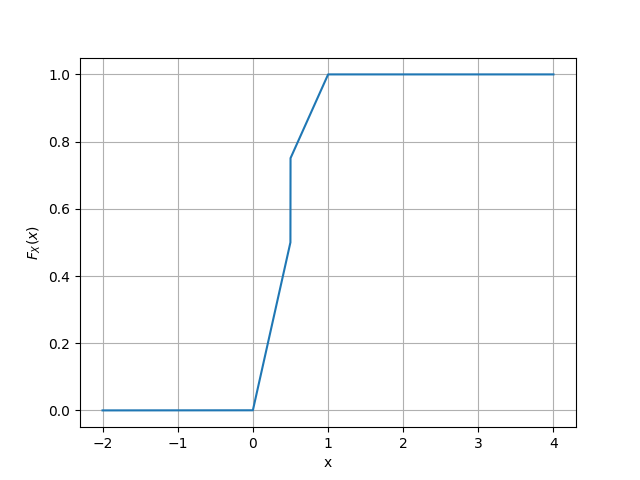
\includegraphics[width=\columnwidth]{solutions/ma/2018/24/cdf_plot.png}
    \caption{cdf plot of random variable X}
    \label{ma2018-24:cdf_plot}
\end{figure}

%
\item Let A and b be two events such that $\pr{B}=\frac{3}{4}$ and $\pr{A + B^{\prime}}=\frac{1}{2}$.If A and B are independent, then $\pr{A}$ equals
\\
\solution
  

Given,
\begin{align}
\pr{B}=\frac{3}{4}\label{st2021-14:a}\\
\pr{A + B^{\prime}} =\frac{1}{2} \label{st2021-14:b}
\end{align}
we know that,
\begin{align}
\pr{B^{\prime}} = 1-\pr{B} \label{st2021-14:c}
\end{align}
using \eqref{st2021-14:a} in \eqref{st2021-14:c},
\begin{align}
\pr{B^{\prime}} = \frac{1}{4} \label{st2021-14:d}
\end{align}
we know that,
\begin{align}
\pr{A + B^{\prime}} = \pr{A} +\pr{B^{\prime}} - \pr{A,B^{\prime}}
\end{align}
A and B are independent $\iff$ A and $B^{\prime}$ are independent
\begin{align}
\pr{A + B^{\prime}} = \pr{A} +\pr{B^{\prime}} - \pr{A}\pr{B^{\prime}} \label{st2021-14:e}
\end{align}
using \eqref{st2021-14:b}  and \eqref{st2021-14:d} in \eqref{st2021-14:e},
\begin{align}
\frac{1}{2} &= \pr{A} + \frac{1}{4} - \frac{\pr{A}}{4}\\
\frac{1}{4} &= \frac{3\pr{A}}{4}\\
\therefore \pr{A} &= \frac{1}{3}
\end{align}
\item Let $(X,Y)$ have a bivariate normal distribution with the joint probability density function
\begin{align}
f_{X,Y}(x,y)=\frac{1}{\pi}e^{(\frac{3}{2}xy-\frac{25}{32}x^2-2y^2)}\\
-\infty < x,y < \infty
\end{align}
Then $E(XY)$ equals 
%
\\
\solution
  
Given probability density function for $(X,Y)$
\begin{align}
f_{X,Y}(x,y)&=\frac{1}{\pi}e^{(\frac{3}{2}xy-\frac{25}{32}x^2-2y^2)} \label{st2021-44:1} \\ 
-\infty &< x,y < \infty
\end{align}
Joint pdf of bivariate normal distribution $N(\mu_x,\mu_y,\sigma_x^2,\sigma_y^2,\rho)$ is
\begin{align}
f_{X,Y}(x,y)&=\frac{1}{2\pi\sigma_x\sigma_y\sqrt{1-p^2}} \times \notag \\ &e^{\frac{-1}{2(1-p^2)}\sbrak{\sbrak{\frac{(x-\mu_x)}{\sigma_x}}^2+\sbrak{\frac{(y-\mu_y)}{\sigma_y}}^2-2\rho\sbrak{\frac{(x-\mu_x)}{\sigma_x}\frac{(y-\mu_y)}{\sigma_y}}}} \label{st2021-44:eq}
\end{align}
Comparing \eqref{st2021-44:eq} and \eqref{st2021-44:1} we get 
\begin{table}[h!]
\resizebox{7cm}{!}
{
\begin{tabular}{|c|c|c|c|c|}
\hline
$\mu_x$ & $\mu_y$ & $\sigma_x$ & $\sigma_y$ & $\rho$ \\
\hline
$0$ & $0$ & $1$ & $\frac{5}{8}$ & $\frac{3}{5}$\\
\hline
\end{tabular}
}
\caption{Table 1} 
\label{st2021-44:tab:1}
\end{table}
We need to find $E(XY)$
\begin{align}
E(XY)&=\rho \sigma_x\sigma_y+\mu_x\mu_y \label{st2021-44:eq:3}
\end{align}
Substituting values in table\eqref{st2021-44:tab:1} in \eqref{st2021-44:eq:3} we get
\begin{align}
E(XY)&=\frac{3}{8} \label{st2021-44:6}\\
\therefore 8E(XY)&=3
\end{align}
%
\item Let $X_{1}$ be	an	exponential	random	variable with mean 1 and $X_{2}$ a gamma	random variable	with mean 2	and	variance 2.	If $X_{1}$ and $X_{2}$ are independently	distributed, then $\pr{X_1 < X_2}$ is equal	to ..........	
\\
\solution
  
We know that,
\begin{align}
    f_{X_1}(x) = 
    \begin{cases}
    0   & x < 0\\
    \lambda e^{\lambda x} & 0\le x < \infty\\
    \end{cases}
\end{align}
Given, 
\begin{align}
   E(X_1)=\cfrac{1}{\lambda}&=1\\ 
   \implies \lambda &=1
\end{align}
Therefore,
\begin{align}
    f_{X_1}(x) = 
    \begin{cases}
    0   & x < 0\\
    e^{-x} & 0\le x < \infty\\
    \end{cases}
\end{align}
We know that,
\begin{align}
    f_{X_2}(x) = 
    \begin{cases}
    0   & x < 0\\
    \cfrac{x^{\alpha-1}e^{\brak{\frac{-x}{\beta}}}}{\beta^{\alpha}\Gamma(\alpha)} & 0\le x < \infty\\
    \end{cases}
\end{align}
Given, 
\begin{equation}\label{ma2016-47:eq:2.0.4}
    E(X_2)=\alpha \beta =2 
\end{equation}
\begin{equation}\label{ma2016-47:eq:2.0.5}
    V(X_2)=\alpha \beta^{2}=2 
\end{equation}
Solving \ref{ma2016-47:eq:2.0.4} and \ref{ma2016-47:eq:2.0.5}, we get,
$\alpha=2$, $\beta=1$ and $\Gamma(2)=1$\\
Therefore,
\begin{align}
    f_{X_2}(x) = 
    \begin{cases}
    0   & x < 0\\
    xe^{-x} & 0\le x < \infty\\
    \end{cases}
\end{align}
Calculating the CDF of $f_{X_2}(x)$,\\
\begin{align}
    F_{X_2}(x)&= \displaystyle\int\limits_0^x f_{X_2}(x)\\
    F_{X_2}(x)&=
    \begin{cases}
    0 & x<0\\
    \cfrac{\gamma(\alpha,\frac{x}{\beta})}{\Gamma(\alpha)} & 0 \le x <\infty
    \end{cases}
\end{align}
For $\alpha=2$ and $\beta=1$\\
Alternately, we have CDF of $X_1$ and $X_2$ given by 
\begin{align}
    F_{X_1}(x) = 
    \begin{cases}
     0   & x < 0\\
    1-e^{-x} & 0\le x < \infty\\
    \end{cases}
\end{align}
\begin{align}
    F_{X_2}(x) = 
    \begin{cases}
    0   & x < 0\\
    \cfrac{\gamma(2,x)}{\Gamma(2)} & 0\le x < \infty\\
    \end{cases}
\end{align}
Thus, 
\begin{align}
    \pr{X_1\le X_2}&=\displaystyle\int\limits_{-\infty}^{\infty} F_{X_1}(x)f_{X_2}(x)dx\\
                &= \displaystyle\int\limits_0^\infty(1-e^{-x})(xe^{-x})dx\\
                &= \cfrac{3}{4}\\
                &= 0.75
\end{align}
%
\item Let $\Omega = (\,0,1]\,$ be the sample space and let $P\brak{.}$ be a probability distribution given by\\
\begin{align}
P\brak{(\,0,x]\,} = 
\begin{cases}
   \frac{x}{2} & 0 \le x < \frac{1}{2}\\
   x & \frac{1}{2} \le x \le 1
\end{cases}
\end{align}
Find $P\brak{\frac{1}{2}}$
\\
\solution
  

CDF of X is defined as,
\begin{align}
    F_X\brak{x}=\pr{X \le x}
\end{align}

$\because x > 0$
\begin{align}
    F_X\brak{x}=P\brak{(\,0,x]\,}
\end{align}
Thus, CDF of $X$ is given by
\begin{align}
    F_X\brak{x} =
    \begin{cases}
    0 & x < 0\\
    \frac{x}{2} & 0 \le x < \frac{1}{2}\\
     x & \frac{1}{2} \le x \le 1\\
     1 & x\geq 1
    \end{cases}
\end{align}
\begin{align}
    \pr{\frac{1}{2}} & = F\brak{\frac{1}{2}} - F\brak{\frac{1}{2}^{-}}\\
    & = \frac{1}{2} - \frac{1/2}{2}\\
    & = \frac{1}{4}
\end{align}
The plot of CDF is given in the Figure \ref{ma2015-27:fig:cdf}

\begin{figure}[h!]
\centering
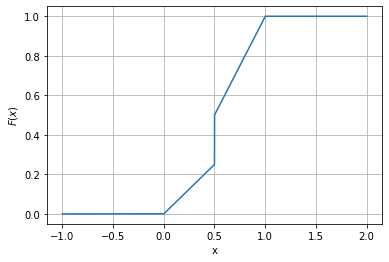
\includegraphics[width=\columnwidth]{solutions/ma/2015/27/Figure/fig4.png}
\caption{CDF of X}
\label{ma2015-27:fig:cdf}
\end{figure}

   


%
\item Let $(X,Y)$ be a two-dimensional random variable such that $E(X)=E(Y)=1/2$, $Var(X)=Var(Y)=1$ and $Cov(X,Y)=1/2$.
Then, $P(|X-Y|>6)$ is
\begin{enumerate}

    \item less than 1/6
    \item equal to 1/2
    \item equal to 1/3
    \item greater than 1/2

\end{enumerate}
\solution
  
Given,
\begin{align} \label{ma2001-24:eq-1}
    E(X)=E(Y)=3
\end{align}
\begin{align}
    Var(X)=Var(Y)=1
\end{align}
\begin{align}
    Cov(X,Y)=1/2
\end{align}
Now,
\begin{align}
    Var(X)=E(X^2)-(E(X))^2
\end{align}
Substituting given values, we get,
\begin{align}
    1=E(X^2)-3^2
\end{align}
So,
\begin{align} \label{ma2001-24:eq-2}
    E(X^2)=10
\end{align}
Similarly for $Y$,
\begin{align} \label{ma2001-24:eq-3}
    E(Y^2)=10
\end{align}
Also,
\begin{align}
    Cov(X,Y)=E(XY)-E(X)E(Y)
\end{align}
Substituting given values, we get,
\begin{align}
    1/2=E(XY)-(3)(3)
\end{align}
So,
\begin{align} \label{ma2001-24:eq-4}
    E(XY)=19/2
\end{align}
Let $Z$ be a random variable defined as
\begin{align} \label{ma2001-24:eq-5}
    Z=X-Y
\end{align}
Then using \eqref{ma2001-24:eq-1},
\begin{align} \label{ma2001-24:eq-6}
    E(Z)=E(X-Y)=E(X)-E(Y)=0
\end{align}
Now, using \eqref{ma2001-24:eq-6}
\begin{align}
    Var(Z)=E(Z^2)-(E(Z))^2=E(Z^2)
\end{align}
\begin{align}
    Var(Z)=E((X-Y)^2)
\end{align}
\begin{align}
    Var(Z)=E(X^2)+E(Y^2)-2E(XY)
\end{align}
Using \eqref{ma2001-24:eq-2}, \eqref{ma2001-24:eq-3} and \eqref{ma2001-24:eq-4},
\begin{align}
    Var(Z)=10+10-2 \times 19/2
\end{align}
\begin{align} \label{ma2001-24:eq-7}
    Var(Z)=1
\end{align}
\begin{theorem}
(Chebychev's Inequality)\ Let T be an arbitrary random variable, with finite mean E(T), then for all $a>0$,
\begin{align}
    \pr{|T-E(T)| \geq a} \leq \dfrac{Var(T)}{a^2}
\end{align}
\end{theorem}
\begin{proof}
Let $A$ be a non-negative random variable and $a>0$ be any real number. Define a new random variable $B$ by
\begin{align}
B=  \begin{cases} 
          a & A \geq a \\
          0 & A < a
    \end{cases}
\end{align}
Then clearly $B \leq A$ and by monotonicity,
\begin{align} \label{ma2001-24:eq-8}
    E(B) \leq E(A)
\end{align}
\begin{align}
    E(B)=a\pr{B=a}+0\pr{B=0}
\end{align}
\begin{align} \label{ma2001-24:eq-9}
    E(B)=a\pr{A \geq a}
\end{align}
By \eqref{ma2001-24:eq-8} and \eqref{ma2001-24:eq-9},
\begin{align}
    a\pr{A \geq a} \leq  E(A)
\end{align}
\begin{align} \label{ma2001-24:eq-10}
    \pr{A \geq a} \leq \dfrac{E(A)}{a}
\end{align}
Set $A=(T-E(T))^2$. Then,
\begin{align}
    \pr{|T-E(T)| \geq a}=\pr{A \geq a^2}
\end{align}
Using \eqref{ma2001-24:eq-10},
\begin{align}
    \pr{|T-E(T)| \geq a} \leq \dfrac{E(A)}{a^2}
\end{align}
\begin{align}
    \pr{|T-E(T)| \geq a} \leq \dfrac{E(T-E(T))^2}{a^2}
\end{align}
\begin{align}
    \pr{|T-E(T)| \geq a} \leq \dfrac{Var(T)}{a^2}
\end{align}
\end{proof}
Applying Chebychev's Inequality for $Z$ with $a=6$, we get,
\begin{align}
    \pr{|Z-E(Z)| \geq 6} \leq \dfrac{Var(Z)}{6^2}
\end{align}
Using \eqref{ma2001-24:eq-6} and \eqref{ma2001-24:eq-7},
\begin{align}
    \pr{|Z-0| \geq 6} \leq \dfrac{1}{36}
\end{align}
As $Z=X-Y$,
\begin{align}
    \pr{|X-Y| \geq 6} \leq \dfrac{1}{36}
\end{align}

\item Let \(X_1,X_2\)... be a sequence of independent and identically distributed random variable with
\begin{align}
    \pr{X_1=-1}=\pr{X_1=1}=1/2
\end{align}
Suppose for the standard normal random variable Z,
\begin{align}
&\pr{-0.1\leq Z \leq 0.1}=0.08 .\label{qneq} \\ \nonumber
&\text{If } S_n= \sum_{i=1}^{n^2} X_i ,\text{then} \lim_{n\to\infty} \pr{S_n >\frac{n}{10}} =
\end{align}
\begin{enumerate}
    \item 0.42
    \item 0.46
    \item 0.50
    \item 0.54
\end{enumerate}
\solution
  
\begin{align}
   &p_{X_i} (n)=\pr{X_i = n}=\nonumber \begin{cases}
            \frac{1}{2}, &\text{if n= 1 or n=-1}\\
             0, &\text{otherwise}\\
            \end{cases} \\ 
    \implies& \mu=E(X_i)=1/2(1-1)=0\\
    \implies& \sigma^2=E({X_i}^2) -\mu^2=\frac{1}{2}(1+1) -0=1
\end{align}
Using Central Limit Theorem,we can say that for a series of random and identical variables \(X_i\) with the \(\text{Mean} =\mu \text{ and variance}=\sigma^2  \)  where i \(\in\) {1,2...n} 
\begin{align}
&\text{Let }\overline{X_n} \equiv \frac{\sum_{i=1}^n X_i}{n}\\
&\text{Then} \lim_{n\to\infty}\sqrt{n}(\overline{X_n}-\mu)=N(0,\sigma^2)\\
&\implies\lim_{n\to\infty}\frac{S_n}{n}=N(0,1)\\
&\implies S_n=n N(0,1)\\
&\implies\lim_{n\to\infty}\pr{n N(0,1) >\frac{n}{10}}\\
&\implies\lim_{n\to\infty} \pr{N(0,1)>\frac{1}{10}}= Q(0.1)\\ \nonumber
&\text{Now using \eqref{qneq}}\\ 
&\implies Q(0.1)+(1-Q(-0.1))+ 0.08=1\\ \nonumber
&\text{Now as }N(0,1) \text{symmetric about 0}\\
&\implies 2\times Q(0.1)+0.08=1\\
&\implies Q(0.1)=0.46\\
&\implies \lim_{n\to\infty} \pr{S_n >\frac{n}{10}}=0.46 
\end{align}
Hence final solution is option 2) or 0.46

\item  Consider an amusement park where visitors are arriving according to a Poisson process with rate 1. Upon arrival, a visitor spends a random amount of time in the park and then departs. The time spent by the visitors is independent of one another, as well as of the arrival process and have common probability density function 
\begin{align}
    f(x) = 
    \begin{cases}
        e^{-x}, & x > 0\\
        0,      & otherwise
    \end{cases}
\end{align}
If at a given point, there are 10 visitors in the park, and p is the probability that there will be exactly two more arrivals before the next departure, then $\frac{1}{p}$ equals.....
\solution
  
According to the question, we want the following events to occur in order: 
\begin{enumerate}
    \item First visitor, $P_1$ arrives while no one leaves
    \item Second visitor $P_2$ arrives while no one leaves
    \item One or more person leaves before the third visitor $P_3$ arrives
\end{enumerate}
Let the above events be $E_1$, $E_2$ and $E_3$ respectively. Thus the required probability
\begin{align}
    &= \pr{E_1E_2E_3}\\
    &= \pr{E_1}\pr{E_2|E_1}\pr{E_3|E_1E_2}\label{st2021-50:Requiredprobability}
\end{align}
\begin{table}
    \centering
    \begin{tabular}{|c|c|}
    \hline
    Symbol  & Representation  \\
    \hline
    $X_1$            & Arrival time of $P_1$  \\
    $X_1+X_2$        & Arrival time of $P_2$  \\
    $X_1+X_2+X_3$    & Arrival time of $P_3$  \\
    \hline
    $Y_1,...,Y_{10}$ & Departure times of the  \\
                     & 10 people in park currently\\
    \hline
    $X_1+Y_{11}$     & Departure time of $P_1$\\
    $X_1+X_2+Y_{12}$ & Departure time of $P_2$\\
    \hline
    \end{tabular}
    \caption{Notations}
    \label{st2021-50:tab:my_label}
\end{table}
First we present the following result which shall be useful later. For $n>0$,
\begin{align}
    \int_0^{\infty} xe^{-nx}dx = \cfrac{1}{n^2}\label{st2021-50:integrationresult}
\end{align}
The above can be derived using integration by parts as follows
\begin{align}
    \int_0^{\infty} xe^{-nx} dx &= -\cfrac{xe^{-nx}}{n} \biggr \vert_0^{\infty} 
                                   + \cfrac{1}{n} \int_0^{\infty}e^{-nx}dx\\
                                &= -\cfrac{e^{-nx}}{n^2}\biggr \vert_0^{\infty}\\
                                &= \cfrac{1}{n^2}
\end{align}
Next we note that $X_1$, $X_2$ and $X_3$ are identical random variables having Poisson distribution with rate 1. Thus for $i \in \{1,2,3\}$,
\begin{align}
    \lambda &= 1*X_i = X_i\\
    k &= 1\\
    \implies f_{X_i}(x) &= 
    \begin{cases}
        \cfrac{x^1e^{-x}}{1!} = x e^{-x} &x > 0\\
        0                                &otherwise
    \end{cases}
\end{align}
Also $Y_1,...,Y_{12}$ are identical random variables. Thus for $i \in \{1,...,12\}$, as given in question,
\begin{align}
    f_{Y_i}(x) &= 
    \begin{cases}
        e^{-x} & x > 0\\
        0      & otherwise
    \end{cases}\\
    \implies F_{Y_i}(x) &= 
    \begin{cases}
        1-e^{-x} & x > 0\\
        0        & otherwise
    \end{cases}
\end{align}
Now we find $\pr{E_1}$, $\pr{E_2|E_1}$ and $\pr{E_3|E_1E_2}$ in order to find the required probability from eq \eqref{st2021-50:Requiredprobability}.
\begin{align}
    \pr{E_1} &= \pr{Y_1,...,Y_{10} > X_1}\\
             &= \int_{-\infty}^{\infty} \pr{Y_1,...,Y_{10} > x|X_1 = x}\\
             &= \int_{-\infty}^{\infty} (1-F_{Y_1}(x))^{10} f_{X_1}(x)dx\\
             &= \int_0^{\infty} xe^{-11x} dx\\
             &= \cfrac{1}{121}
\end{align}
\begin{multline}
    \pr{E_2|E_1} =\\
    \pr{Y_1,...,Y_{10},X_1+Y_{11} > X_1 + X_2|Y_1,...,Y_{10} > X_1}
\end{multline}
Using memoryless property of exponential random variable,
\begin{align}
    \pr{E_2|E_1} &= \pr{Y_1,...,Y_{11} > X_2}\\
                 &= \int_{-\infty}^{\infty} \pr{Y_1,...Y_{11} > x|X_2 = x}\\
                 &= \int_{-\infty}^{\infty} (1-F_{Y_1}(x))^{11} f_{X_2}(x)dx\\
                 &= \int_{0}^{\infty} x e^{-12x} dx\\
                 &= \cfrac{1}{144}
\end{align}
$\pr{E_3|E_1E_2} = $  
\begin{multline}
    \Pr(min(Y_1,...,Y_{10},X_1+Y_{11},X_1+X_2+Y_{12}) \\
    < X_1+X_2+X_3| Y_1,...,Y_{10},X_1+Y_{11} > X_1+X_2)
\end{multline}
We can simplify and write $\pr{E_3|E_1E_2} = $
\begin{multline}
    1 - \Pr(Y_1,...,Y_{10},X_1+Y_{11},X_1+X_2+Y_{12} \\
    > X_1+X_2+X_3| Y_1,...,Y_{10},X_1+Y_{11} > X_1+X_2)
\end{multline}
Using memoryless property of exponential random variable,
\begin{align}
    \pr{E_3|E_1E_2} &= 1 - \pr{Y_1,...,Y_{12} > X_3}\\
                    &= 1 - \int_{-\infty}^{\infty} \pr{Y_1,...Y_{12} > x|X_3 = x}\\
                    &= 1 - \int_{-\infty}^{\infty} (1-F_{Y_1}(x))^{12} f_{X_3}(x)dx\\
                    &= 1 - \int_{0}^{\infty} x e^{-13x} dx\\
                    &= 1 - \cfrac{1}{169}\\
                    &= \cfrac{168}{169}
\end{align}
Thus on substituting values in \eqref{st2021-50:Requiredprobability}, 
\begin{align}
    \pr{E_1E_2E_3} &= \cfrac{1}{121}\times \cfrac{1}{144}\times \cfrac{168}{169}\\
                   &= 5.7 \times 10^{-5}
\end{align}

\item  Let $\{X_n\}_{n\ge 1}$ be a sequence of independent and identically distributed random variables each having uniform distribution on [0,3]. Let $Y$ be a random variable, independent of $\{X_n\}_{n\ge 1}$, having probability mass function
\begin{align}
\pr{Y=k} = 
\begin{cases}
\frac{1}{(e-1)k!} & k=1,2,3\cdots \\
0 & otherwise
\end{cases}
\end{align}
Then $\pr{max\{X_1,X_2,\cdots X_Y\}\le 1}$ equals ............\\
%
\solution
  
Given that $\{X_n\}_{n\ge 1}$ is having a uniform distribution on [0,3], so probability can be written as
\begin{align}
\pr{X_n}_{n\ge 1}=  
\begin{cases}
\frac{1}{3} & 0\le X_n\le 3 \\
0 & otherwise
\end{cases}
\end{align}
So,
\begin{align}
    \pr{X_n\le 1}_{n\ge 1}=\frac{1}{3}
\end{align}
Required probability
\begin{align}
 &=\pr{max\{X_1,X_2,\cdots X_Y\}\le 1}\label{st2021-48:req_prob}
 \end{align}
 Since, $\{X_n\}_{n\ge 1}$ is a sequence of independent variables and $Y$ is also independent of $\{X_n\}_{n\ge 1}$.\\
 And also in \eqref{st2021-48:req_prob}, the index of $X_i's$ depends on $Y$, so number of terms depends on $Y$, like if $Y=1$, then there is only $X_1$, if $Y=2$, then there's $X_1,X_2$, so required probability
\begin{align}
&=\sum_{p=1}^{\infty}\pr{max\{X_1,X_2,\cdots X_p\}\le 1|Y=p}\cdot \pr{Y=p}
\end{align}
\begin{align}
& =\sum_{p=1}^{\infty}\pr{max\{X_1,X_2,\cdots X_p\}\le 1}\cdot \pr{Y=p}\\
&=\sum_{p=1}^{\infty}\pr{X_1,X_2,\cdots X_p\le 1}\cdot \pr{Y=p}
\end{align}
\begin{multline}
=\sum_{p=1}^{\infty}\pr{X_1\le 1}\cdot \pr{X_2\le 1}\cdots \pr{X_{p-1}\le 1}\\
\cdot \pr{X_p\le 1}\cdot \pr{Y=p}
\end{multline}
\begin{align}
&=\sum_{p=1}^{\infty}\left(\frac{1}{3}\right)^p\left(\frac{1}{e-1}\right)\left(\frac{1}{p!}\right)\\
&=\left(\frac{1}{e-1}\right)\left[\sum_{p=0}^{\infty}\left(\frac{1}{3}\right)^p\left(\frac{1}{p!}\right)-1\right]
\label{st2021-48:taylor}
\end{align}
Using Taylor's Series of $e^x$ in \eqref{st2021-48:taylor}, \\
Required probability
\begin{align}
    &=\frac{e^{1/3}}{e-1}-\frac{1}{e-1}\\
    &=0.23
\end{align}
    


\item The characteristic function of a random variable X is given by
\begin{align}
\phi_{X}\brak{t}
=
\begin{cases}
\frac{\sin{t}\cos{t}}{t}           & t \neq 0 \\
1        & t = 0
\end{cases}
\end{align}
Then $ P\brak{|X|\leq \frac{3}{2}} =$ 
%
\solution
  
The pdf is given by
\begin{align}
    f_{X}(x) = \frac{1}{2\pi} \int_{-\infty}^{\infty}  \phi_{X}\brak{t}e^{-jxt} dt 
\end{align}
If
\begin{align}
    g\brak{x} &\system{F} G\brak{t}\\
    \implies G\brak{t} &\system{F} g\brak{-x} \label{st2020-16:th}
\end{align}
where $ \brak{\system{F}}$ represents Fourier transform and
\begin{align}
    G\brak{t}  = \int_{-\infty}^{\infty} g\brak{x} e^{-j2\pi xt} dx 
\end{align}
we know that the Fourier transform of rectangular function is sinc function
\begin{align}
    rect\brak{\frac{x}{\tau}} &\system{F} \tau sinc(t\tau)
\end{align}
from \eqref{st2020-16:th} we get
\begin{align}
  \tau sinc(t\tau) &\system{F} rect\brak{-\frac{x}{\tau}}
\end{align}
\begin{align}
 \implies rect\brak{-\frac{x}{\tau}} = \int_{-\infty}^{\infty} \tau \frac{\sin{\pi t \tau}}{{\pi t \tau}} e^{-j2\pi xt}dt
\end{align}
substituting $\tau = \frac{2}{\pi}$ and changing $2\pi x \rightarrow x $ we get
\begin{align}
    \frac{1}{4}rect\brak{\frac{-x}{4}} = \frac{1}{2\pi} \int_{-\infty}^{\infty} \brak {\frac{\sin{2t}}{2t}}e^{-jxt} dt 
\end{align}
So
\begin{align}
    f_{X}(x) &= \frac{1}{4}rect\brak{\frac{-x}{4}}\\
    P\brak{|X|\leq \frac{3}{2}} &= \int_{\frac{-3}{2}}^{\frac{3}{2}} \frac{1}{4} dx\\
    &=\frac{3}{4}
\end{align}
\begin{figure}[!ht]
\centering
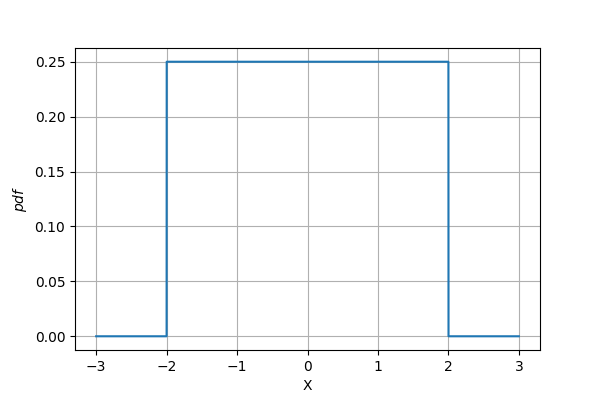
\includegraphics[width=\columnwidth]{solutions/st/2020/16/figs/Assignment5.png}
\caption{$f_{X}(x)$}
\label{st2020-16:pdf}
\end{figure}



% %
% \item Let $\{X_j\}$ be a sequence of independent Bernoulli random variables with $\mathbb{P}(X_j=1) = \frac{1}{4}$ and let $Y_n = \frac{1}{n} \sum_{j=1}^{n}X_j^2$. Then $Y_n$ converges, in probability, to $\rule{2cm}{0.15mm}$ .
% %
% \solution
%   
A sequence of random variables $Y_1,Y_2,Y_3\hdots$ converges, in probability, to a random variable $Y$ if
\begin{align}
    \lim_{n\rightarrow \infty}\Pr{(\abs{Y_n-Y}\geq \epsilon)} = 0 \quad \forall \epsilon >0
\end{align}
Similarly, a sequence of random variables $Y_1,Y_2,Y_3\hdots$ converges, in mean square, to a random variable $Y$ if
\begin{align}
    \lim_{n\rightarrow \infty} E(\abs{Y_n-Y}^2) = 0 
\end{align}
A random variable converges, in probability, to a value if it converges, in mean square, to the same particular value by Markov's Inequality. Proof for this is: For any $\epsilon > 0$
\begin{align}
    \Pr{(\abs{Y_n-Y}\geq \epsilon)} = \Pr{(\abs{Y_n-Y}^2\geq \epsilon^2)}
\end{align}
\begin{multline}
    \Pr{(\abs{Y_n-Y}\geq \epsilon)}  \leq \frac{E\abs{Y_n-Y}^2}{\epsilon^2} 
    \\\text{ (by Markov's Inequality)}
\end{multline}
 
\begin{align}
    \lim_{n\rightarrow \infty} E(\abs{Y_n-Y}^2) = 0 
    \\0 \leq  \lim_{n\rightarrow \infty}\Pr{(\abs{Y_n-Y}\geq \epsilon)}  \leq \frac{0}{\epsilon^2}
    \\   \lim_{n\rightarrow \infty}\Pr{(\abs{Y_n-Y}\geq \epsilon)} = 0 \quad \forall \epsilon >0
\end{align}
Given in the question that $\{X_j\}$ is a sequence of random variables with
\begin{align}
    \Pr{(X_j=1)} = \frac{1}{4}
    \\\Pr{(X_j=0)} + \Pr{(X_j=1)} = 1
    \\\Pr{(X_j=0)} = 1 - \frac{1}{4} = \frac{3}{4}
\end{align}
\begin{align}
    X_j \in \{0,1\} 
\end{align}
Since $0^2 = 0$ and $1^2 = 1$, 
\begin{align}
    X_j^2 = X_j \quad \forall j \in \{1, 2,\hdots, n\}
\end{align}
Thus, 
\begin{align}
    Y_n &= \frac{1}{n} \sum_{j=1}^{n}X_j^2 
    \\&= \frac{1}{n} \sum_{j=1}^{n}X_j
    \\\Pr{(Y_n = y)} &= \comb{n}{ny} \brak{\frac{1}{4}}^{ny} \brak{\frac{3}{4}}^{n-ny}
\end{align}
Let us assume
\begin{align}
    k &= ny
    \\k &\in \{0,1,2,\hdots,n-1,n\}
    \\ \Pr{(Y_n = \frac{k}{n})} &= \comb{n}{k} \brak{\frac{1}{4}}^{k} \brak{\frac{3}{4}}^{n-k}
\end{align}
\begin{align}
    E\brak{\abs{Y_n-\frac{1}{4}}^2} &= E\brak{Y_n^2 - \frac{1}{2}Y_n + \frac{1}{16}}
    \\&= E(Y_n^2) - \frac{1}{2}E(Y_n) + \frac{1}{16} \label{ma2018-25:equation 0}
\end{align}
\begin{align}
    E(Y_n^2) &= \sum_{k=0}^n\brak{\frac{k}{n}}^2\Pr{\brak{Y_n=\frac{k}{n}}}
    \\&= \sum_{k=0}^{n} \brak{\frac{k^2}{n^2}}\comb{n}{k} \brak{\frac{1}{4}}^{k} \brak{\frac{3}{4}}^{n-k}
\end{align}
\begin{multline}
    E(Y_n^2) = 0 + \frac{1}{n^2}\times n\brak{\frac{1}{4}}^{1} \brak{\frac{3}{4}}^{n-1} + \\\sum_{k=2}^{n} \brak{\frac{k}{n}}^2\times\frac{n(n-1)}{k(k-1)}
    \times\comb{n-2}{k-2}\brak{\frac{1}{4}}^{k} \brak{\frac{3}{4}}^{n-k}
\end{multline}
\begin{multline}
    E(Y_n^2) =  \frac{1}{4n}\brak{\frac{3}{4}}^{n-1} + \frac{n-1}{n} 
   \\\times\sum_{k=2}^{n} \brak{\frac{k}{k-1}}\comb{n-2}{k-2}\brak{\frac{1}{4}}^{k} \brak{\frac{3}{4}}^{n-k}
\end{multline}
\begin{multline}
    E(Y_n^2)  = \frac{1}{4n}\brak{\frac{3}{4}}^{n-1} \\+ \frac{n-1}{n} 
   \brak{\sum_{k=2}^{n}\comb{n-2}{k-2}\brak{\frac{1}{4}}^{k} \brak{\frac{3}{4}}^{n-k} }
   \\+\frac{n-1}{n} \brak{\sum_{k=2}^{n}\frac{1}{k-1}\comb{n-2}{k-2}\brak{\frac{1}{4}}^{k} \brak{\frac{3}{4}}^{n-k} } 
\end{multline}
\begin{multline}
    E(Y_n^2)  = \frac{1}{4n}\brak{\frac{3}{4}}^{n-1} + \frac{n-1}{n}\\ \times\frac{1}{16} 
   \brak{\sum_{k=2}^{n}\comb{n-2}{k-2}\brak{\frac{1}{4}}^{k-2} \brak{\frac{3}{4}}^{(n-2)-(k-2)} }
   \\+\frac{1}{n} \brak{\sum_{k=2}^{n}\frac{n-1}{k-1}\comb{n-2}{k-2}\brak{\frac{1}{4}}^{k} \brak{\frac{3}{4}}^{n-k} }
\end{multline}
\begin{multline}
     E(Y_n^2)= \frac{1}{4n}\brak{\frac{3}{4}}^{n-1} \\+ \frac{n-1}{16n} 
   \brak{\sum_{j=0}^{n-2}\comb{n-2}{j}\brak{\frac{1}{4}}^{j} \brak{\frac{3}{4}}^{(n-2)-j} }
   \\+\frac{1}{4n} \brak{\sum_{k=2}^{n}\comb{n-1}{k-1}\brak{\frac{1}{4}}^{k-1} \brak{\frac{3}{4}}^{(n-1)-(k-1)} } 
\end{multline}
\begin{multline}
    E(Y_n^2) = \frac{1}{4n}\brak{\frac{3}{4}}^{n-1} + \frac{n-1}{16n}\brak{\frac{1}{4} + \frac{3}{4}}^{n-2}
   \\+\frac{1}{4n} \brak{\sum_{j=1}^{n-1}\comb{n-1}{j}\brak{\frac{1}{4}}^{j} \brak{\frac{3}{4}}^{(n-1)-j} }
\end{multline}
\begin{multline}
   E(Y_n^2) = \frac{1}{4n}\brak{\frac{3}{4}}^{n-1} + \frac{n-1}{16n}
   \\+\frac{1}{4n} \brak{\brak{\frac{1}{4} + \frac{3}{4}}^{n-1} - \brak{\frac{3}{4}}^{n-1}} 
\end{multline}
\begin{align}
    E(Y_n^2) &= \frac{1}{4n}\brak{\frac{3}{4}}^{n-1} + \frac{n-1}{16n} +\frac{1}{4n} - \frac{1}{4n}\brak{\frac{3}{4}}^{n-1}
    \\&= \frac{1}{16} + \frac{3}{16n} \label{ma2018-25:equation 2}
\end{align}
\begin{align}
    E(Y_n) &= \sum_{k=0}^n\frac{k}{n}\Pr{\brak{Y_n=\frac{k}{n}}}
    \\&= \sum_{k=0}^{n} \brak{\frac{k}{n}}\comb{n}{k} \brak{\frac{1}{4}}^{k} \brak{\frac{3}{4}}^{n-k}
    \\&= 0 + \sum_{k=1}^{n} \frac{k}{n}\times\frac{n}{k}\times\comb{n-1}{k-1}\brak{\frac{1}{4}}^{k} \brak{\frac{3}{4}}^{n-k}
    \\&= \frac{1}{4}\sum_{j=0}^{n-1} \comb{n-1}{j}\brak{\frac{1}{4}}^{j} \brak{\frac{3}{4}}^{(n-1)-j}
    \\&= \frac{1}{4}\brak{\frac{1}{4} + \frac{3}{4}}^{n-1}
    \\&= \frac{1}{4} \label{ma2018-25:equation 3}
\end{align}
Using equations \eqref{ma2018-25:equation 2} and \eqref{ma2018-25:equation 3} in \eqref{ma2018-25:equation 0},
\begin{align}
    E\brak{\abs{Y_n-\frac{1}{4}}^2} &= \frac{1}{16}+ \frac{3}{16n}-\frac{1}{2}\times\frac{1}{4} + \frac{1}{16}
    \\&= \frac{3}{16n}
\end{align}
\begin{align}
    \lim_{n\rightarrow \infty} E\brak{\abs{Y_n-\frac{1}{4}}^2} &=  \lim_{n\rightarrow \infty}  \frac{3}{16n}
    \\&= \frac{3}{16}\lim_{n\rightarrow \infty}\frac{1}{n}
    \\&= 0
\end{align}
Thus, $Y_n$ converges, in mean square, to $\frac{1}{4}$ and hence $Y_n$ converges, in probability, to $\frac{1}{4}$.

%
\item Let $\{X_j\}$ be a sequence of independent Bernoulli random variables with $\mathbb{P}(X_j=1) = \frac{1}{4}$ and let $Y_n = \frac{1}{n} \sum_{j=1}^{n}X_j^2$. Then $Y_n$ converges, in probability, to $\rule{2cm}{0.15mm}$ .
\solution
  
A sequence of random variables $Y_1,Y_2,Y_3\hdots$ converges, in probability, to a random variable $Y$ if
\begin{align}
    \lim_{n\rightarrow \infty}\Pr{(\abs{Y_n-Y}\geq \epsilon)} = 0 \quad \forall \epsilon >0
\end{align}
Similarly, a sequence of random variables $Y_1,Y_2,Y_3\hdots$ converges, in mean square, to a random variable $Y$ if
\begin{align}
    \lim_{n\rightarrow \infty} E(\abs{Y_n-Y}^2) = 0 
\end{align}
A random variable converges, in probability, to a value if it converges, in mean square, to the same particular value by Markov's Inequality. Proof for this is: For any $\epsilon > 0$
\begin{align}
    \Pr{(\abs{Y_n-Y}\geq \epsilon)} = \Pr{(\abs{Y_n-Y}^2\geq \epsilon^2)}
\end{align}
\begin{multline}
    \Pr{(\abs{Y_n-Y}\geq \epsilon)}  \leq \frac{E\abs{Y_n-Y}^2}{\epsilon^2} 
    \\\text{ (by Markov's Inequality)}
\end{multline}
 
\begin{align}
    \lim_{n\rightarrow \infty} E(\abs{Y_n-Y}^2) = 0 
    \\0 \leq  \lim_{n\rightarrow \infty}\Pr{(\abs{Y_n-Y}\geq \epsilon)}  \leq \frac{0}{\epsilon^2}
    \\   \lim_{n\rightarrow \infty}\Pr{(\abs{Y_n-Y}\geq \epsilon)} = 0 \quad \forall \epsilon >0
\end{align}
Given in the question that $\{X_j\}$ is a sequence of random variables with
\begin{align}
    \Pr{(X_j=1)} = \frac{1}{4}
    \\\Pr{(X_j=0)} + \Pr{(X_j=1)} = 1
    \\\Pr{(X_j=0)} = 1 - \frac{1}{4} = \frac{3}{4}
\end{align}
\begin{align}
    X_j \in \{0,1\} 
\end{align}
Since $0^2 = 0$ and $1^2 = 1$, 
\begin{align}
    X_j^2 = X_j \quad \forall j \in \{1, 2,\hdots, n\}
\end{align}
Thus, 
\begin{align}
    Y_n &= \frac{1}{n} \sum_{j=1}^{n}X_j^2 
    \\&= \frac{1}{n} \sum_{j=1}^{n}X_j
    \\\Pr{(Y_n = y)} &= \comb{n}{ny} \brak{\frac{1}{4}}^{ny} \brak{\frac{3}{4}}^{n-ny}
\end{align}
Let us assume
\begin{align}
    k &= ny
    \\k &\in \{0,1,2,\hdots,n-1,n\}
    \\ \Pr{(Y_n = \frac{k}{n})} &= \comb{n}{k} \brak{\frac{1}{4}}^{k} \brak{\frac{3}{4}}^{n-k}
\end{align}
\begin{align}
    E\brak{\abs{Y_n-\frac{1}{4}}^2} &= E\brak{Y_n^2 - \frac{1}{2}Y_n + \frac{1}{16}}
    \\&= E(Y_n^2) - \frac{1}{2}E(Y_n) + \frac{1}{16} \label{ma2018-25:equation 0}
\end{align}
\begin{align}
    E(Y_n^2) &= \sum_{k=0}^n\brak{\frac{k}{n}}^2\Pr{\brak{Y_n=\frac{k}{n}}}
    \\&= \sum_{k=0}^{n} \brak{\frac{k^2}{n^2}}\comb{n}{k} \brak{\frac{1}{4}}^{k} \brak{\frac{3}{4}}^{n-k}
\end{align}
\begin{multline}
    E(Y_n^2) = 0 + \frac{1}{n^2}\times n\brak{\frac{1}{4}}^{1} \brak{\frac{3}{4}}^{n-1} + \\\sum_{k=2}^{n} \brak{\frac{k}{n}}^2\times\frac{n(n-1)}{k(k-1)}
    \times\comb{n-2}{k-2}\brak{\frac{1}{4}}^{k} \brak{\frac{3}{4}}^{n-k}
\end{multline}
\begin{multline}
    E(Y_n^2) =  \frac{1}{4n}\brak{\frac{3}{4}}^{n-1} + \frac{n-1}{n} 
   \\\times\sum_{k=2}^{n} \brak{\frac{k}{k-1}}\comb{n-2}{k-2}\brak{\frac{1}{4}}^{k} \brak{\frac{3}{4}}^{n-k}
\end{multline}
\begin{multline}
    E(Y_n^2)  = \frac{1}{4n}\brak{\frac{3}{4}}^{n-1} \\+ \frac{n-1}{n} 
   \brak{\sum_{k=2}^{n}\comb{n-2}{k-2}\brak{\frac{1}{4}}^{k} \brak{\frac{3}{4}}^{n-k} }
   \\+\frac{n-1}{n} \brak{\sum_{k=2}^{n}\frac{1}{k-1}\comb{n-2}{k-2}\brak{\frac{1}{4}}^{k} \brak{\frac{3}{4}}^{n-k} } 
\end{multline}
\begin{multline}
    E(Y_n^2)  = \frac{1}{4n}\brak{\frac{3}{4}}^{n-1} + \frac{n-1}{n}\\ \times\frac{1}{16} 
   \brak{\sum_{k=2}^{n}\comb{n-2}{k-2}\brak{\frac{1}{4}}^{k-2} \brak{\frac{3}{4}}^{(n-2)-(k-2)} }
   \\+\frac{1}{n} \brak{\sum_{k=2}^{n}\frac{n-1}{k-1}\comb{n-2}{k-2}\brak{\frac{1}{4}}^{k} \brak{\frac{3}{4}}^{n-k} }
\end{multline}
\begin{multline}
     E(Y_n^2)= \frac{1}{4n}\brak{\frac{3}{4}}^{n-1} \\+ \frac{n-1}{16n} 
   \brak{\sum_{j=0}^{n-2}\comb{n-2}{j}\brak{\frac{1}{4}}^{j} \brak{\frac{3}{4}}^{(n-2)-j} }
   \\+\frac{1}{4n} \brak{\sum_{k=2}^{n}\comb{n-1}{k-1}\brak{\frac{1}{4}}^{k-1} \brak{\frac{3}{4}}^{(n-1)-(k-1)} } 
\end{multline}
\begin{multline}
    E(Y_n^2) = \frac{1}{4n}\brak{\frac{3}{4}}^{n-1} + \frac{n-1}{16n}\brak{\frac{1}{4} + \frac{3}{4}}^{n-2}
   \\+\frac{1}{4n} \brak{\sum_{j=1}^{n-1}\comb{n-1}{j}\brak{\frac{1}{4}}^{j} \brak{\frac{3}{4}}^{(n-1)-j} }
\end{multline}
\begin{multline}
   E(Y_n^2) = \frac{1}{4n}\brak{\frac{3}{4}}^{n-1} + \frac{n-1}{16n}
   \\+\frac{1}{4n} \brak{\brak{\frac{1}{4} + \frac{3}{4}}^{n-1} - \brak{\frac{3}{4}}^{n-1}} 
\end{multline}
\begin{align}
    E(Y_n^2) &= \frac{1}{4n}\brak{\frac{3}{4}}^{n-1} + \frac{n-1}{16n} +\frac{1}{4n} - \frac{1}{4n}\brak{\frac{3}{4}}^{n-1}
    \\&= \frac{1}{16} + \frac{3}{16n} \label{ma2018-25:equation 2}
\end{align}
\begin{align}
    E(Y_n) &= \sum_{k=0}^n\frac{k}{n}\Pr{\brak{Y_n=\frac{k}{n}}}
    \\&= \sum_{k=0}^{n} \brak{\frac{k}{n}}\comb{n}{k} \brak{\frac{1}{4}}^{k} \brak{\frac{3}{4}}^{n-k}
    \\&= 0 + \sum_{k=1}^{n} \frac{k}{n}\times\frac{n}{k}\times\comb{n-1}{k-1}\brak{\frac{1}{4}}^{k} \brak{\frac{3}{4}}^{n-k}
    \\&= \frac{1}{4}\sum_{j=0}^{n-1} \comb{n-1}{j}\brak{\frac{1}{4}}^{j} \brak{\frac{3}{4}}^{(n-1)-j}
    \\&= \frac{1}{4}\brak{\frac{1}{4} + \frac{3}{4}}^{n-1}
    \\&= \frac{1}{4} \label{ma2018-25:equation 3}
\end{align}
Using equations \eqref{ma2018-25:equation 2} and \eqref{ma2018-25:equation 3} in \eqref{ma2018-25:equation 0},
\begin{align}
    E\brak{\abs{Y_n-\frac{1}{4}}^2} &= \frac{1}{16}+ \frac{3}{16n}-\frac{1}{2}\times\frac{1}{4} + \frac{1}{16}
    \\&= \frac{3}{16n}
\end{align}
\begin{align}
    \lim_{n\rightarrow \infty} E\brak{\abs{Y_n-\frac{1}{4}}^2} &=  \lim_{n\rightarrow \infty}  \frac{3}{16n}
    \\&= \frac{3}{16}\lim_{n\rightarrow \infty}\frac{1}{n}
    \\&= 0
\end{align}
Thus, $Y_n$ converges, in mean square, to $\frac{1}{4}$ and hence $Y_n$ converges, in probability, to $\frac{1}{4}$.
%
\item The variable $x$ takes a value between $0$ and $10$ with uniform probability distribution. The variable $y$ takes a value between $0$ and $20$ with uniform probability distribution.The probability that sum of variables $(x+y)$ being greater than $20$ is
%
\item Robot Ltd. wishes to maintain enough safety
stock during the lead time period between
starting a new production run and its completion
such that the probability of satisfying the
customer demand during the lead time period
is 95\%. The lead time periods is 5 days and
daily customer demand can be assumed to follow
the Gaussian (normal) distribution with mean
50 units and a standard deviation of 10 units.
Using $\phi^{-1}$(0.95) =1.64 , where $\phi$ represents the
cumulative distribution function of the standard
normal random variable, the amount of safety
stock that must be maintained by Robot Ltd. to
achieve this demand fulfillment probability for
the lead time period is \rule{1cm}{0.15mm}  units (round off to
two decimal places).
%
\solution
  
\begin{table}[htp]
\centering
    \resizebox{\columnwidth}{15mm}{
\begin{tabular}{ |c|c|c|c|} 
\hline
Symbol & definition & value \\
\hline
X &customer demand in lead time& -\\
\hline
$X_1$ &normal R.V denotes daily customer demand & -\\
\hline
$\mu$ & Mean of $X_1$& 50 \\
\hline
$\sigma$ & Standard deviation of $X_1$ & 10\\
\hline
$\phi$ &CDF of standard normal R.V& -\\
\hline
\end{tabular}}
\caption{Variables and their definitions}
\label{me2021-20:table1}
\end{table}
Probability of satisfying customer demand is 0.95.
Let Z be a standard normal R.V such that,
\begin{align}
    Z=\frac{X_1-\mu}{\sigma} \label{me2021-20:3}
\end{align}
Referring table\eqref{me2021-20:table1} to use in \eqref{me2021-20:3},
\begin{align}
    Z=\frac{X_1-50}{10}\label{me2021-20:4}
\end{align}
Given that,
\begin{align}
    \phi^{-1}(0.95)&=1.64\\
    \implies \phi(1.64)&=0.95\\
    \phi(1.64)&=\pr{Z\le1.64}=0.95\\
    \implies Z\le1.64&\iff\frac{X_1-50}{10}\le1.64\\
    \implies X_1-50 &\le 1.64(10)\\
    \therefore X_1\le66.4
\end{align}
The demand in one day is independent of demand in the other day and the lead time is 5 days.
\begin{align}
    \implies X=5(X_1)=5(66.4)=332
\end{align}
Therefore the amount of safety
stock that must be maintained by Robot Ltd. to
achieve this demand fulfillment probability for
the lead time period is 332 units.
%
% \item 
% Probability density function $p(x)$ of random variable x is as shown below. The value of a is
% \begin{enumerate}[label=\Alph*)]
%     \item $\frac{2}{c}$
%     \item $\frac{1}{c}$
%     \item $\frac{2}{(b+c)}$
%     \item $\frac{1}{(b+c)}$
% \end{enumerate}
% \begin{figure}[h!]
% \centering
% \includegraphics[width=\columnwidth]{solutions/in/2006/2/figures/convolution.png}
% \caption{PDF}
% \label{in2006-2:fig:BSC}
% \end{figure}
% %
% \solution
%   

Let $Y_1$ and $Y_2$ be two independent and identically distributed (IID) uniform random variables.\\
Let X be a random variable such that
\begin{align}
    X = Y_1 + Y_2
\end{align}
Let
\begin{align}
    p_{Y_1}\brak{y} &= \Pr\brak{Y_1=y} \\
    p_{Y_2}\brak{y} &= \Pr\brak{Y_2=y} \\
    p_X\brak{x} &= \Pr\brak{X=x}
\end{align}
be the probability densities of random variables $Y_1, Y_2$ and $X$. \\
$Y_1$ and $Y_2$ lie in the range \brak{\frac{-c}{4},\frac{c}{4}}, therefore, the PDF for $Y_1$ and $Y_2$,
\begin{align}
p_{Y_1}\brak{y} = p_{Y_2}\brak{y} = 
\begin{cases}
\frac{2}{c} &  \frac{-c}{4} \le y \le \frac{c}{4}\\
0 & \text{otherwise}
\end{cases}
\end{align}

The density of X is obtained by convolution of $Y_1$ and $Y_2$
\begin{align}
p_X\brak{x} = p_{Y_1}(x)*p_{Y_2}(x)
\end{align}
where $*$ denotes the convolution operation. Since convolution operation is time invariant, 
\begin{multline}
    p_X\brak{x-t} = p_{Y_1}(x-t)*p_{Y_2}(x) \\ = p_{Y_1}(x)*p_{Y_2}(x-t)
\end{multline}
On time shifting $Y_1$ by shifting factor $t=a+\frac{c}{2}$, 
\begin{align}
    p_X\brak{x-\brak{a+\frac{c}{2}}} =  p_{Y_1}\brak{x-\brak{a+\frac{c}{2}}}*p_{Y_2}\brak{x}
\end{align}
Thus, the PDF of time shifted X obtained by convolution is,
\begin{align}
p_x = 
\begin{cases}
\frac{4}{c^2}\brak{x-a} & a \le x \le a+\frac{c}{2}\\
\frac{4}{c^2}\brak{a+c-x} & a+\frac{c}{2} \le x \le a+c \\
0 & \text{otherwise}
\end{cases}
\end{align}

On comparing the parameters of PDF of time shifted X with that in the question, we have

\begin{align}
    b=\frac{c}{2}\\
    a=\frac{2}{c}
\end{align}
\rightline{Answer : Option A}


\begin{figure}[!ht]
\centering
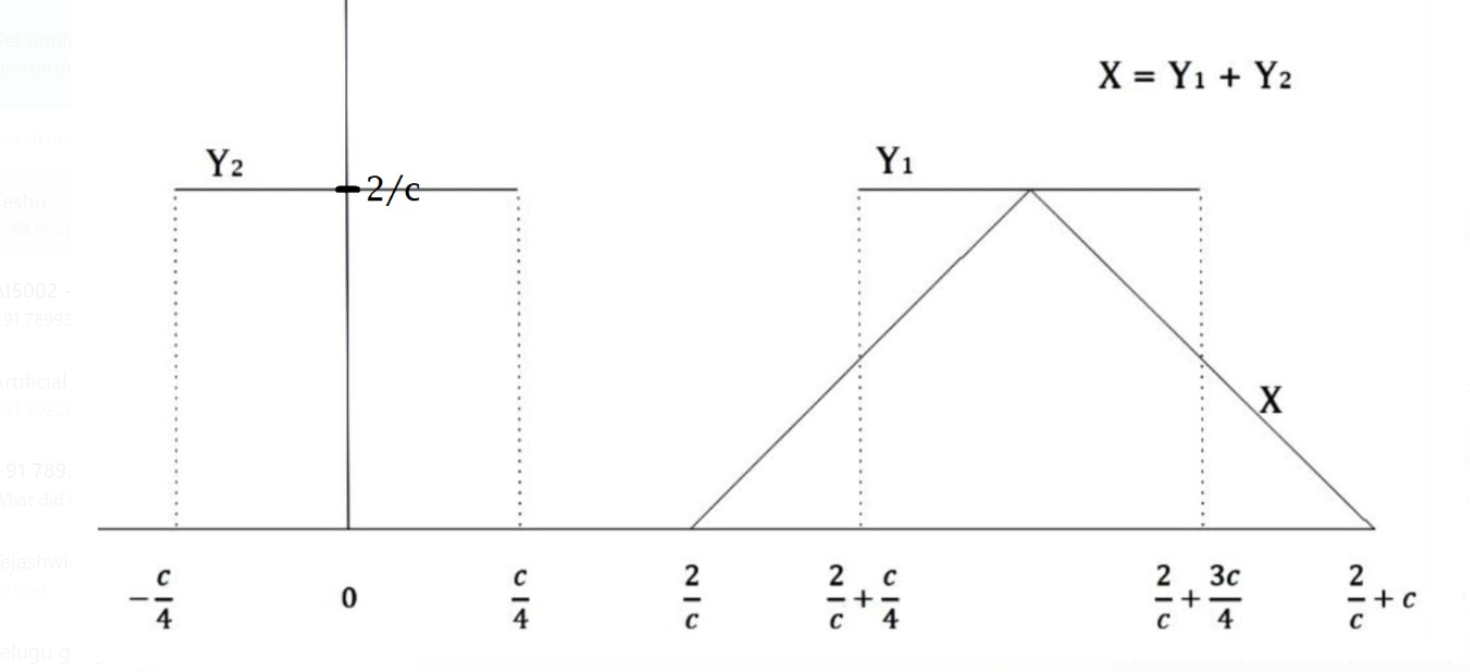
\includegraphics[width=\columnwidth]{solutions/in/2006/2/figures/con6.png}
\caption{PDF of time shifted X}
\label{in2006-2:fig:convolution}
\end{figure}
The following are some observations: 
\begin{enumerate}
    \item The sum of two equally distributed random variables will lead to a triangular probability density
    \item The two uniformly distributed random variables lie in the range $\brak{\frac{-c}{4},\frac{c}{4}}$ and $\brak{\frac{2}{c}+\frac{c}{4} , \frac{2}{c}+\frac{3c}{4}}$. \\
    \because $X = Y_1 + Y_2$ the range of X is thus $\brak{\frac{2}{c},\frac{2}{c}+c}$
    \item On time shifting $Y_1$ to the right by a factor $a+\frac{c}{2}$, the convoluted PDF of X also shifts by the same factor without any change in it's width.
\end{enumerate}

Fig \ref{in2006-2:fig:sim1} and Fig \ref{in2006-2:fig:sim2} are the simulated plots of PDF and CDF obtained by taking c=2
\begin{figure}[h!]
\centering
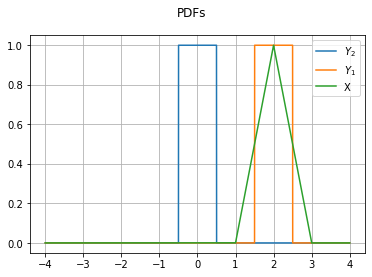
\includegraphics[width=\columnwidth]{solutions/in/2006/2/figures/sim1.png}
\caption{PDF of $Y_1, Y_2$ and X}
\label{in2006-2:fig:sim1}
\end{figure}
\begin{figure}[!ht]
\centering
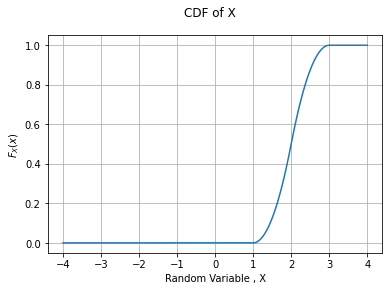
\includegraphics[width=\columnwidth]{solutions/in/2006/2/figures/sim2.png}
\caption{CDF of X}
\label{in2006-2:fig:sim2}
\end{figure}


\end{document}

% %
\item Let X be a random variable having probability density function 
\begin{align}
\label{st2021-22:eq:qpdf_X}
f\brak{x} = 
\begin{cases}
\frac{3}{13}(1-x)(9-x) & 0 < x < 1
\\
0 & \text{ otherwise}
\end{cases}
\end{align}
Then $\dfrac{4}{3} E [X(X^2 -15X + 27 ) ] $ equals --- ( round of to two decimal places). \\
\solution
  
Let X be the random variable. To find 
\begin{align}
    \frac{4}{3} E[X(X^2 -15X + 27)]
\end{align}
Let,
\begin{align}
    g(X) &= X(X^2 -15X + 27)  \\
         &= X^3 -15X^2 + 27X
\end{align}
Then for random variable X we have that,
\begin{align}
    E[g(X)] = \int_{-\infty}^{\infty} g(x)f(x) \,dx
\end{align}
The probability distribution of X is,
\begin{align}
\label{st2021-22:eq:spdf_X}
f\brak{x} = 
\begin{cases}
\frac{3}{13}(1-x)(9-x) & 0 < x < 1
\\
0 & \text{ otherwise}
\end{cases}
\end{align}
Using \ref{st2021-22:eq:spdf_X} we have,
\begin{align}
    E[g(X)] &= 0 +\int_{0}^{1} g(x)f(x) \,dx + 0
\end{align}
Where ,
\begin{align}
    f(x ) &= \frac{3}{13}(1-x)(9-x) \text{ and}  \\
    g(x) &= x^3 -15x^2 + 27x
\end{align}
Using Integration by substitution let,
\begin{align*}
    t &= x^3 - 15x^2 + 27x \\
    \,dt &= 3x^2 - 30x + 27 \\
         &= 3(1-x)(9-x)
\end{align*}
The corresponding limits are,
\begin{align}
    \text{For } x &=0  \implies t = 0^3 -15\times 0^2 + 27 \times 0 = 0 \\
        \text{For } x &=1  \implies t = 1^3 -15\times 1^2 + 27 \times 1 = 13
\end{align}
Therefore we have,
\begin{align}
    E[g(X)] &= \frac{1}{13} \int_{0}^{13} t \,dt \\
    & = \frac{1}{13} \times \brak{\frac{t^2}{2}}  \Biggr|_{0}^{13} \\
    &= \frac{1}{13} \times \frac{13^2}{2} \\
    & = \frac{13}{2} 
\end{align}
Thus, 
\begin{align}
    \frac{4}{3} E[g(X)] & =  \frac{4}{3} \times \frac{13}{2} \\
    &= \frac{26}{3} \\
    &= 8.67  \text{ (rounded off)}
\end{align}
Therefore,
\begin{align}
    \frac{4}{3} E[X(X^2 -15X + 27)] & =  8.67
\end{align}
%
\item Two independent events E and F are such that $P(E\cap F) = \displaystyle\frac{1}{6}$,$P(E^c\cap F^c)=\displaystyle\frac{1}{3}$ and $P(E)>P(F)$. Then $P(E)$ is
\begin{enumerate}[label=(\Alph*)]
    \item $\displaystyle\frac{1}{2}$\\
    \item $\displaystyle\frac{2}{3}$\\
    \item $\displaystyle\frac{1}{3}$\\
    \item $\displaystyle\frac{1}{4}$
\end{enumerate}
%
\solution
  
If E and F are independent, E' and F' are also independent.\\So,
\begin{align}
    \pr{EF}&=\pr{E}\pr{F}\nonumber\\
            &=\frac{1}{6}\label{ma1999-28:a}\\
    \pr{E'F'}&=\pr{E'}\pr{F'}\nonumber\\
            &=\brak{1-\pr{E}}\brak{1-\pr{F}}\nonumber\\
            &=\frac{1}{3}\label{ma1999-28:c}
\end{align}
From $\eqref{ma1999-28:a}$ and $\eqref{ma1999-28:c}$
\begin{align}
    \pr{E}+\pr{F}&=\frac{5}{6}\label{ma1999-28:b}
\end{align}
From $\eqref{ma1999-28:a}$ and $\eqref{ma1999-28:b}$,
\begin{align}
    \pr{E}\brak{\frac{5}{6}-\pr{E}}&=\frac{1}{6}\nonumber\\
\equiv \pr{E}&=\frac{1}{3}\text{or}\frac{1}{2}\nonumber
\end{align}
$\pr{E}=\frac{1}{2}$ satisfies $\pr{E}>\pr{F}$ while $\pr{E}=\frac{1}{3}$ does not.\\
$\therefore \pr{E}=\frac{1}{2}$\\
\solution{Option A}
%
\item Let $Y_{1},Y_{2},...,Y_{15}$ be a random sample of size 15 from the probability density function 
\begin{align}
\tag{Eq:1}
    f_{y}(y)=3(1-y)^{2} , 0<y<1
\end{align}
Use the central limit theorem to approximate $P\brak{\frac{1}{8}<\Bar{Y}<\frac{3}{8}}$
%
\solution
  
The \textbf{central limit theorem} states that whenever a random sample of size n is taken from any distribution with mean and variance, then the sample mean will be approximately normally distributed with mean and variance. The larger the value of the sample size, the better the approximation to the normal.
\begin{align}
\tag{1.1}
    Z_{n}=\frac{\bar{Y}-\mu}{\frac{\sigma}{\sqrt{n}}}
    \label{ma1996-25:eq:1}
\end{align}
From equation \ref{ma1996-25:eq:1}
\begin{align}
    \tag{1.2}
    \bar{Y}=Z_{n}\brak{\frac{\sigma}{\sqrt{n}}}+\mu
\end{align}
\begin{align}
\tag{1.3}
\pr{\frac{1}{8}<\Bar{Y}<\frac{3}{8}}
&=\pr{\frac{1}{8}<Z_{n}\brak{\frac{\sigma}{\sqrt{n}}}+\mu<\frac{3}{8}}\\
\tag{1.4}  
&=\pr{\frac{\frac{1}{8}-\mu}{\frac{\sigma}{\sqrt{n}}}<Z_{n}<\frac{\frac{3}{8}-\mu}{\frac{\sigma}{\sqrt{n}}}}
\label{ma1996-25:eq;123}
\end{align}
$\bar{Y}$:Mean of the randomly selected 15 variables
\begin{align}
\tag{1.5}
    \bar{Y}=\frac{Y_{1}+Y_{2}+..Y_{15}}{15}
\end{align}
Mean of probability density function is
\begin{align}
\tag{1.6}
\mu&=\int_{-\infty}^{\infty}yf(y)dy\\
\tag{1.7}
    &=\int_{0}^{1}y\times 3(1-y)^{2}dy\\
\tag{1.8}
    &=\frac{1}{4}
\end{align}
Variance of probability density function is
\begin{align}
\tag{1.9}
\sigma^{2}&=E[y^{2}]-(E[y])^{2}\\
\tag{1.10}
\label{ma1996-25:eq;2}
      &=\brak{\int_{0}^{1}y^{2}f(y)dy} - \brak{\frac{1}{4}}^{2}
\end{align}
\begin{align}
\tag{1.11}
    \int_{0}^{1}y^{2}f(y)dy &= \int_{0}^{1}y^{2}\times3(1-y)^{2}dy\\
\tag{1.12}
                            &=3\int_{0}^{1}(y-y^{2})^{2}dy\\
\tag{1.13}
\label{ma1996-25:eq;3}
                            &=\frac{1}{10}
\end{align}
Substituting equation \ref{ma1996-25:eq;3} in equation \ref{ma1996-25:eq;2}
\begin{align}
\tag{1.14}
 \sigma^{2}&=\frac{1}{10}-\frac{1}{16}\\
\tag{1.15}
           &=\frac{3}{80}
\end{align}
Using Q function in equation \ref{ma1996-25:eq;123} we have,
\begin{align}
\notag
\pr{\frac{1}{8}<\Bar{Y}<\frac{3}{8}}
&=\pr{\frac{\frac{1}{8}-\mu}{\frac{\sigma}{\sqrt{n}}}<Z_{n}<\frac{\frac{3}{8}-\mu}{\frac{\sigma}{\sqrt{n}}}}\\
\tag{1.16}
&=\pr{\frac{\frac{1}{8}-\mu(y)}{\frac{\sigma}{\sqrt{n}}}<Z_{n}<\frac{\frac{3}{8}-\mu(y)}{\frac{\sigma}{\sqrt{n}}}}\\
\tag{1.17}
&=Q\brak{\frac{\frac{-1}{8}}{\sqrt{\frac{3}{80}}}}-Q\brak{\frac{\frac{1}{8}}{\sqrt{\frac{3}{80}}}}\\
\tag{1.18}
&=1-2Q\brak{\frac{\frac{1}{8}}{\sqrt{\frac{3}{80}}}}\\
\tag{1.19}                             
&=1-2Q\brak{0.645}\\
\tag{1.20}                             
&=0.9938
\end{align}


\end{enumerate}
\end{document}
